% (c) 2012 Tiziana Manca - tmanca@libero.it
% (c) 2012 - 2014 Dimitrios Vrettos - d.vrettos@gmail.com

\chapter{Relazioni}
%===================================
\section{Proposizioni e predicati}
In matematica frasi come ``19 è maggiore di~5'' o ``Giove ruota intorno alla Terra'' sono considerate \emph{proposizioni} perché ad esse
si può attribuire un preciso valore di verità, cioè si può stabilire se sono vere oppure false: la prima è una proposizione vera, la seconda è falsa.

Non sono proposizioni in senso matematico ``Cosa stai studiando?'', ``domani pioverà!'', ``$x$ è un numero primo'':
infatti la prima non è un'affermazione ma pone una domanda, la seconda è una esclamazione e quindi non possiamo stabilire se è vera o falsa;
l'ultima contiene un elemento indeterminato e finché non si fissa il valore da attribuire a~$x$, non si può decidere se la frase che lo riguarda è vera o falsa.

Ogni proposizione è formata da un \emph{predicato} (verbo) e dai suoi \emph{argomenti} (cose o persone alle quali il verbo si riferisce).

Analizzando le proposizioni sopra enunciate si ha:
\begin{center}
\begin{tabular}{llc}
\toprule
Soggetto & Predicato & Complemento \\
\midrule
19 & è maggiore di & 5 \\
Giove & ruota attorno alla & Terra \\
\bottomrule
\end{tabular}
\end{center}
Il soggetto e il complemento sono gli argomenti ai quali il predicato si riferisce.
In alcune proposizioni il predicato si riferisce a due argomenti (il \emph{soggetto} e il \emph{complemento})
in altre ad un solo argomento: ad esempio, il predicato ``essere numero primo'' stabilisce semplicemente una caratteristica del numero~5
senza porre alcuna connessione con un altro argomento.

\begin{definizione}\label{def:predicato_binario}
Si dice \emph{predicato binario} un predicato che si riferisce a due argomenti.
\end{definizione}

\ovalbox{\risolvi \ref{ese:B.1}}

\section{Relazioni in un insieme}

Il termine \emph{relazione} entra molto spesso in frasi del linguaggio naturale, lo usiamo per esprimere un generico legame tra due persone o tra due oggetti,
anche senza specificarne la natura: ``si è conclusa la relazione tra Anna e Paolo'', ``l'allungamento di una sbarretta di ferro è in relazione con il calore fornito'',
``la frana del terreno è in relazione con il disboscamento della zona e l'abusivismo edilizio'', ``domani consegnerò la relazione di fisica''.
Sono tutte espressioni che ci danno informazioni di un qualche collegamento tra gli
argomenti (persone, cose) ai quali il termine relazione si riferisce.

Dal punto di vista matematico diamo la seguente definizione.
\begin{definizione}
Si dice \emph{relazione} in un insieme~$A$ un predicato binario che lega due elementi dell'insieme.
\end{definizione}

\begin{exrig}
 \begin{esempio}
 Nell'insieme~$A = \{3\text{,~}5\text{,~}6\text{,~}9\text{,~}30\}$ è introdotto il predicato binario ``essere multiplo di''; con esso formiamo le proposizioni vere scegliendo soggetto e
 complemento nell'insieme~$A$:

\begin{multicols}{3}
30 è multiplo di~6;

9 è multiplo di~3;

30 è multiplo di~3;

6 è multiplo di~3;

30 è multiplo di~5;

3 è multiplo di~3;

5 è multiplo di~5;

6 è multiplo di~6;

9 è multiplo di~9;

30 è multiplo di~30.
\end{multicols}
Il predicato ``essere multiplo'' genera nell'insieme~$A$ una relazione matematica. Esso tuttavia non è il
solo che permette di collegare tra loro due elementi di quell'insieme.
\end{esempio}
\end{exrig}

\ovalbox{\risolvi \ref{ese:B.2}}

Se chiamiamo con~$\Rel$ il predicato binario che definisce la relazione introdotta nell'insieme, per indicare 
sinteticamente la proposizione avente come soggetto~$a$, come complemento~$b$ e come predicato~$\Rel$, scriviamo~$a \,\Rel\, b$ e
diremo che~\emph{$a$ è in relazione con~$b$}.

\begin{exrig}
 \begin{esempio}

Con riferimento all'esempio precedente si ha:~$A = \{3\text{,~}5\text{,~}6\text{,~}9\text{,~}30\}$ e $\Rel$:
``essere multiplo di''. Allora scriviamo: per qualunque~$a$ e~$b$ appartenenti ad~$A$,
$a \,\Rel\, b$ se e solo se~$a$ è multiplo di~$b$, in particolare:
\[30 \,\Rel\,~6;\quad~9 \,\Rel\,~3;\quad~30 \,\Rel\,~3;\quad~6 \,\Rel\,~3;\quad~30 \,\Rel\,~5;\quad~3 \,\Rel\,~3;\quad 5 \,\Rel\,~5;\quad~6 \,\Rel\,~6;\quad~9 \,\Rel\,~9;\quad~30 \,\Rel\,~30.\]
\end{esempio}
\end{exrig}

Abbiamo così formato un insieme di coppie ordinate di elementi tra loro in relazione:~$30 \,\Rel\,~5$ può anche essere indicata con la coppia ordinata~$(30;5)$.

\begin{definizione}
Chiamiamo \emph{insieme della relazione} $G_\Rel$ l'insieme delle coppie ordinate i cui
elementi sono gli argomenti del predicato binario, ossia sono in relazione tra di loro. Esso risulta essere un
sottoinsieme del prodotto cartesiano dell'insieme~$A$ con se stesso. Si rappresenta per proprietà caratteristica nel
seguente modo~$G_\Rel = \{(a;b) \in A \times A \mid  a \,\Rel\, b \}$.
\end{definizione}

\ovalbox{\risolvii \ref{ese:B.3}, \ref{ese:B.4}, \ref{ese:B.5}, \ref{ese:B.6}}
%===================================
\subsection{Grafico di una relazione}

Dal momento che una relazione in un insieme~$Y$ determina un sottoinsieme del prodotto cartesiano~$Y \times Y$, è
comodo rappresentare una relazione nello stesso diagramma usato per rappresentare il prodotto cartesiano.
Una relazione può quindi essere rappresentata attraverso un \emph{grafico cartesiano}.

\ovalbox{\risolvii \ref{ese:B.7}, \ref{ese:B.8}}

%===================================
\subsection{Matrice o tabella di una relazione}

Nella figura~\ref{fig:B.1} è rappresentata la classica griglia per il gioco della battaglia navale.
Ogni cella è individuata da una coppia ordinata il cui primo elemento (una lettera dell'alfabeto) indica la riga,
il secondo (un numero) indica la colonna; così la coppia~$(D;5)$ indica la cella annerita.

\ovalbox{\risolvii \ref{ese:B.9}, \ref{ese:B.10}, \ref{ese:B.11}}

%===================================
\subsection{Grafo di una relazione}

\begin{definizione}
Un \emph{grafo} è un insieme di punti, detti \emph{nodi}, e di archi che uniscono coppie di punti.
\end{definizione}

Abbiamo visto che con un predicato si possono formare alcune proposizioni aventi rispettivamente come soggetto e
come complemento elementi di un insieme: solo le proposizioni vere determinano la relazione tra gli elementi di
quell'insieme e generano coppie di elementi in relazione.

\begin{exrig}
 \begin{esempio}

Nel diagramma di Eulero-Venn di figura~\ref{fig:B.2}, relativo all'insieme~$A = \{$3, 5, 6, 9, 30$\}$
rappresentiamo la relazione~$\Rel$ = ``essere multiplo di'' collegando, mediante una freccia, gli argomenti delle proposizione vere.

Come puoi osservare, l'elemento~30 è collegato con una freccia all'elemento~6 in quanto la proposizione ``30 è multiplo di~6'' è vera, ma non all'elemento~9
poiché la proposizione ``30 è multiplo di~9'' è falsa; inoltre la punta della freccia è sul numero~6 in quanto complemento del predicato ``essere multiplo di'' (si parla in tal caso di \emph{grafo orientato});
infine su ciascun elemento abbiamo messo un ``anello'' o ``cappio'' per indicare che ogni elemento è in relazione con se stesso visto che per ogni
elemento~$a \in A$ la proposizione ``$a$ è multiplo di~$a$'' risulta vera.

 \end{esempio}
\end{exrig}

\ovalbox{\risolvii \ref{ese:B.12}, \ref{ese:B.13}, \ref{ese:B.14}, \ref{ese:B.15}, \ref{ese:B.16}, \ref{ese:B.17}, \ref{ese:B.18}}
\begin{figure}[hb]
\begin{minipage}[t]{.45\textwidth}
 \centering
 % (c) 2012 Dimitrios Vrettos - d.vrettos@gmail.com

\begin{tikzpicture}[x=10mm,y=10mm, font=\small,table nodes/.style={%
		rectangle,
		draw=black,
 		align=center,
   		minimum height=5mm,
     	text depth=0.5ex,
     	text height=1.5ex,
     	inner xsep=-1pt,
     	outer sep=0pt
	},
	table/.style={%
        matrix of nodes,
        row sep=-\pgflinewidth,
        column sep=-\pgflinewidth,
        nodes={%
            table nodes
        },
        execute at empty cell={\node[fill=black]{};}
    }]

\matrix (first) [table,text width=7mm,name=table]
{
{}  & 1 & 2 & 3 &4 & 5 & 6 & 7\\
$A$ &{} &{} &{} &{} &{} &{} &{} \\
$B$ &{} &{} &{} &{} &{} &{} &{} \\
$C$ &{} &{} &{} &{} &{} &{} &{} \\
$D$ &{} &{} &{} &{} & &{} &{}  \\
$E$ &{} &{} &{} &{} &{} &{} &{} \\
$F$ &{} &{} &{} &{} &{} &{} &{} \\
};

\end{tikzpicture}

 \caption{Griglia della battaglia navale.}\label{fig:B.1}
\end{minipage}\hfil
\begin{minipage}[t]{.45\textwidth}
 \centering
 % (c) 2012 Dimitrios Vrettos - d.vrettos@gmail.com

\begin{tikzpicture}[x=10mm,y=10mm, font=\small, every state/.style={draw=CornflowerBlue}, every loop/.style={draw=Maroon}]
\draw (0,0) circle (2);

\node[state] (5) at (-1.5,0) {5};
\node[state] (30) at (-.4,.8) {30};
\node[state] (6) at (1.1,.5) {6};
\node[state] (9) at (1,-1) {9};
\node[state] (3) at (-.5,-1.2) {3};

\begin{scope}[->]
\path(5) edge[loop below] node{} ()
	(30) edge[loop above] node{} ()
	(6) edge[loop above] node{} ()
	(9) edge[loop above] node{} ()
	(3) edge[loop left] node{} ();

\end{scope}
\begin{scope}[->, Maroon]
\draw (30)--(5);
\draw (30)--(6);
\draw (30)--(3);
\draw (6)--(3);
\draw (9)--(3);
\end{scope}
\end{tikzpicture}

 \caption{L'insieme~$A$.}\label{fig:B.2}
\end{minipage}
\end{figure}

\pagebreak
\section{Proprietà delle relazioni}
%===================================
\subsection{Proprietà riflessiva}

\begin{exrig}
 \begin{esempio}

Nell'insieme~$T = \{\text{7, 8, 12, 34, 100}\}$ è introdotta la relazione~$\Rel$: ``essere divisore di''.
Puoi verificare che ogni numero è divisore di se stesso, cioè ogni elemento dell'insieme è in relazione
con se stesso. Una relazione di questo tipo si dice che gode della \emph{proprietà riflessiva}.
Osserva, però, che nell'insieme ~$\insN$ dei numeri naturali la relazione ``essere divisibile per'' non è riflessiva poiché zero non è divisibile per se stesso.
 \end{esempio}
\end{exrig}

\begin{definizione}
Una relazione~$\Rel$ in un insieme~$A$ gode della \emph{proprietà riflessiva} quando ogni elemento è in relazione con se stesso, ossia per qualunque~$x$ dell'insieme~$A$ si ha~$x \,\Rel\, x$.
\end{definizione}

\ovalbox{\risolvi \ref{ese:B.19}}

%===================================
\subsection{Proprietà antiriflessiva}

\begin{exrig}
 \begin{esempio}
Nell'insieme delle persone~$P = \{\text{Marco, Antonio, Carlo}\}$ è data la relazione~$\Rel$: ``essere più alto di''
rappresentata con la figura~\ref{fig:B.3} di pagina~\pageref{fig:B.3}.
Puoi notare che nessun elemento è in relazione con se stesso. In effetti nessuno può essere più alto di se stesso.

 \end{esempio}
\end{exrig}

\begin{definizione}
Una relazione~$\Rel$ in un insieme~$A$ gode della \emph{proprietà antiriflessiva} quando nessun elemento è in relazione con se stesso,
ossia per nessun elemento~$x$ di~$A$ si ha~$x \,\Rel\, x$.
\end{definizione}

\ovalbox{\risolvi \ref{ese:B.20}}
\subsection{Proprietà simmetrica}

\begin{exrig}
 \begin{esempio}
Nella figura~\ref{fig:B.4} a pagina~\pageref{fig:B.4} è rappresentata la relazione~$\Rel$: ``essere concorde con'' nell'insieme dei numeri~$A = \{-1\text{, }+3\text{, }-7\text{, }+5\text{, }-2\text{, }+4\text{, }+10\}$.
Per collegare elementi in relazione abbiamo usato archi anziché frecce poiché, ad esempio, le proposizioni ``$+3$ è concorde con~$+10$'' e ``$+10$ è concorde con~$+3$''
sono entrambe vere. Per questa relazione si può osservare che se un elemento dell'insieme è in relazione con un altro allora anche quest'ultimo è in relazione con il primo:
$-1 \,\Rel\, -7$, ma anche~$-7 \,\Rel\, -1$; $+3 \,\Rel\, +5$, ma anche~$+5 \,\Rel\, +3$ e così via.
 \end{esempio}
\end{exrig}

\begin{figure}[ht]
\begin{minipage}[t]{.45\textwidth}
 \centering
 % (c) 2012 Dimitrios Vrettos - d.vrettos@gmail.com

\begin{tikzpicture}[x=10mm,y=10mm, font=\small, every state/.style={draw=CornflowerBlue}, every loop/.style={draw=Maroon}]
\draw (0,0) circle (1.8);

\node at (1.8,1.5) {$P$};

\node[state] (M) at (-1,.3) {$M$};
\node[state] (C) at (.8,.8) {$C$};
\node[state] (A) at (.2,-1) {$A$};

 \begin{scope}[->, Maroon]
 \draw (M)--(C);
 \draw (M)--(A);
 \draw (C)--(A);
 \end{scope}
\end{tikzpicture}
 \caption{Proprietà antiriflessiva.}\label{fig:B.3}
\end{minipage}\hfil
\begin{minipage}[t]{.45\textwidth}
 \centering
 % (c) 2012 Dimitrios Vrettos - d.vrettos@gmail.com

\begin{tikzpicture}[x=10mm,y=10mm, font=\small, every state/.style={draw=CornflowerBlue}, every loop/.style={draw=Maroon}]
\draw (0,0) circle [x radius=3, y radius=2];

\node[state] (A) at (-2.3,.3) {$-1$};
\node[state] (B) at (-.8,1.2) {$-2$};
\node[state] (C) at (-1.5,-1) {$-7$};
\node[state] (D) at (-.5,-.9) {$+10$};
\node[state] (E) at (.6,.9) {$+3$};
\node[state] (F) at (1.8,.5) {$+4$};
\node[state] (G) at (1.5,-1) {$+5$};

\begin{scope}[->]
\path(A) edge[loop below] node{} ()
	(B) edge[loop right] node{} ()
	(C) edge[loop left] node{} ()	
(D) edge[loop below] node{} ()
	(E) edge[loop above] node{} ()
	(F) edge[loop right] node{} ()
	(G) edge[loop right] node{} ();

\end{scope}
% \begin{scope}[<->, Maroon]
 \begin{scope}[-, Maroon]
 \draw (A)--(C);
 \draw (B)--(A);
 \draw (C)--(B);
\draw (D)--(E);
\draw (D)--(F);
\draw (E)--(F);
\draw (G)--(F);
\draw (E)--(G);
\draw (D)--(G);
 \end{scope}
\end{tikzpicture}

 \caption{Proprietà simmetrica.}\label{fig:B.4}
\end{minipage}
\end{figure}

\begin{definizione}
Una relazione~$\Rel$ in un insieme~$A$ gode della \emph{proprietà simmetrica} quando risultano vere le due proposizioni
che si ottengono scambiando soggetto e complemento; ossia per qualunque~$x$ e~$y$ appartenenti all'insieme~$A$ se vale~$x \,\Rel\, y$
allora vale anche~$y \,\Rel\, x$.
\end{definizione}

\ovalbox{\risolvi \ref{ese:B.21}}

%===================================
\subsection{Proprietà antisimmetrica}

\begin{exrig}
 \begin{esempio}

Il diagramma di Venn nella figura~\ref{fig:B.5} rappresenta un insieme~$U$ e alcuni suoi sottoinsiemi.

Consideriamo ora l'insieme di insiemi~$S = \{U\text{,~}A\text{,~}B\text{,~}C\text{,~}D\text{,~}E\text{,~}F\}$ e la relazione~$\Rel$: ``essere sottoinsieme proprio di''.
Completa il grafo della relazione.

Certamente nel completare il grafo (figura~\ref{fig:B.6}) non avrai usato archi poiché è evidente che le proposizioni ``$B$ è sottoinsieme proprio di~$C$'' e ``$C$
è sottoinsieme proprio di~$B$'' non possono essere entrambe vere. Anzi, la verità della prima implica necessariamente la falsità della seconda.
 \end{esempio}
\end{exrig}

\begin{figure}[hb]
\begin{minipage}[b]{.45\textwidth}
 \centering
 % (c) 2012 Dimitrios Vrettos - d.vrettos@gmail.com

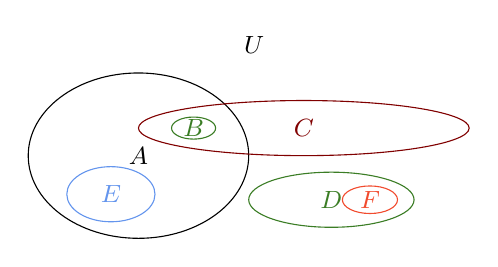
\begin{tikzpicture}[scale=.7,x=10mm,y=10mm, font=\small, every state/.style={draw=CornflowerBlue}, every loop/.style={draw=Maroon}]
\draw (0,0) circle [x radius=2, y radius=1.5] node {$A$};
\draw[CornflowerBlue] (-.5,-.7) circle [x radius=.8, y radius=.5]node {$E$};
\draw[OliveGreen] (1,.5) circle [x radius=.4, y radius=.2]node {$B$};
\draw[Maroon] (3,.5) circle [x radius=3, y radius=.5]node {$C$};
\draw[OliveGreen] (3.5,-.8) circle [x radius=1.5, y radius=.5]node {$D$};
\draw[RedOrange] (4.2,-.8) circle [x radius=.5, y radius=.25]node {$F$};

\node () at (2.1,2) {$U$};
\end{tikzpicture}
 \caption{L'insieme~$U$.}\label{fig:B.5}
\end{minipage}\hfil
\begin{minipage}[b]{.45\textwidth}
 \centering
 % (c) 2012 Dimitrios Vrettos - d.vrettos@gmail.com

\begin{tikzpicture}[scale=.7,x=10mm,y=10mm, font=\small, every state/.style={draw=CornflowerBlue}, every loop/.style={draw=Maroon}]
\draw (0,0) circle [x radius=3, y radius=2];

\node at (3,1.5) {$S$};
\node[state] (A) at (-2.3,.3) {$A$};
\node[state] (B) at (-.8,1.2) {$B$};
\node[state] (C) at (-1.5,-1) {$C$};
\node[state] (D) at (-.2,-1.1) {$D$};
\node[state] (E) at (.6,.9) {$E$};
\node[state] (F) at (1.8,.5) {$F$};
\node[state] (U) at (1.5,-1) {$U$};

  \begin{scope}[->, Maroon]
 \draw (A)--(U);
  \draw (B)--(C);
 \draw (F)--(U);
   \end{scope}
\end{tikzpicture}
 \caption{L'insieme~$S$.}\label{fig:B.6}
\end{minipage}
\end{figure}

\begin{definizione}
Una relazione~$\Rel$ in un insieme~$A$ gode della \emph{proprietà antisimmetrica} quando non possono essere vere
contemporaneamente le proposizioni che si ottengono scambiando il soggetto con il complemento, se soggetto e complemento sono diversi
tra loro; ossia per qualunque~$x$ e~$y$ dell'insieme~$A$ se~$x \neq y$ e se~$x \,\Rel\, y$ non è vero che~$y \,\Rel\, x$.
\end{definizione}

\ovalbox{\risolvi \ref{ese:B.22}}

%===================================
\subsection{Proprietà transitiva}

\begin{exrig}
 \begin{esempio}

Nel grafo di figura~\ref{fig:B.7} è rappresentata una relazione~$\Rel$ introdotta in un insieme~$T$. Dall'analisi della situazione rappresentata possiamo
affermare che dalla verità di $a \,\Rel\, b$ e~$b \,\Rel\, c$ segue la verità di~$a \,\Rel\, c$. Analizzando gli altri elementi, 
possiamo osservare che essendo vere $e \,\Rel\, f$ e~$f\, \Rel\, g$ è vera anche~$e \,\Rel\, g$;
inoltre si ha che essendo vera $n \,\Rel\, m$ e~$m \,\Rel\, t$ è vera anche~$n \,\Rel\, t$.
 \end{esempio}
\end{exrig}

\begin{figure}[ht]
\begin{minipage}[b]{.45\textwidth}
 \centering
 % (c) 2012 Dimitrios Vrettos - d.vrettos@gmail.com

\begin{tikzpicture}[x=10mm,y=10mm, font=\small, every state/.style={draw=CornflowerBlue}, every loop/.style={draw=Maroon}]
\draw (0,0) circle [x radius=3, y radius=2];

\node at (3,1.5) {$T$};
\node[state] (A) at (-2.3,.3) {$a$};
\node[state] (B) at (-.8,1.2) {$b$};
\node[state] (C) at (-1,0) {$c$};
\node[state] (G) at (.2,0) {$g$};
\node[state] (E) at (.6,1.3) {$e$};
\node[state] (F) at (1.8,.8) {$f$};
\node[state] (M) at (1.5,-1.1) {$m$};
\node[state] (N) at (0,-1.2) {$n$};
\node[state] (T) at (2.2,-.2) {$t$};
\begin{scope}[->, Maroon]
\draw (A)--(C);
\draw (B)--(C);
\draw (A)--(B);

\draw (E)--(F);
\draw (E)--(G);
\draw (F)--(G);

\draw (N)--(M);
\draw (N)--(T);
\draw (M)--(T);
\end{scope}
\end{tikzpicture}
 \caption{L'insieme~$T$.}\label{fig:B.7}
\end{minipage}\hfil
\begin{minipage}[b]{.45\textwidth}
 \centering
 % (c) 2012 Dimitrios Vrettos - d.vrettos@gmail.com

\begin{tikzpicture}[x=10mm,y=10mm, font=\small, every state/.style={draw=CornflowerBlue}, every loop/.style={draw=Maroon}]
\draw (0,0) circle [x radius=3, y radius=2];

\node at (3,1.5) {$B$};
\node[state] (A) at (-2.3,.3) {$a$};
\node[state] (H) at (-.8,1.2) {$h$};
\node[state] (F) at (-1.5,-1) {$f$};
\node[state] (B) at (-.5,-.3) {$b$};
\node[state] (E) at (.6,.9) {$e$};
\node[state] (C) at (1.8,.5) {$c$};
\node[state] (D) at (1.5,-.5) {$d$};
\node[state] (G) at (.5,-1.3) {$g$};
\begin{scope}[->]
\path(A) edge[loop below] node{} ()
(H) edge[loop right] node{} ()
(F) edge[loop left] node{} ()	
(B) edge[loop below] node{} ()
(E) edge[loop above] node{} ()
(C) edge[loop right] node{} ()
(D) edge[loop right] node{} ()
(G) edge[loop above] node{} ();
\end{scope}
\begin{scope}[-, Maroon]
\draw (A)--(H);
\draw (F)--(A);
\draw (F)--(H);
\draw (B)--(E);
\draw (B)--(C);
\draw (E)--(C);
\draw (G)--(D);
\end{scope}
\end{tikzpicture}
 \caption{L'insieme~$B$.}\label{fig:B.8}
\end{minipage}
\end{figure}

\begin{definizione}
Una relazione~$\Rel$ in un insieme~$A$ gode della \emph{proprietà transitiva} quando se~$a \,\Rel\, b$ e~$b \,\Rel\, c$
allora risulta anche~$a \,\Rel\, c$, con~$a$, $b$, $c$ elementi qualsiasi dell'insieme~$A$.
\end{definizione}

\ovalbox{\risolvii \ref{ese:B.23}, \ref{ese:B.24}, \ref{ese:B.25}, \ref{ese:B.26}, \ref{ese:B.27}, \ref{ese:B.28}, \ref{ese:B.29}}

%===================================
\section{Relazioni di equivalenza}

\begin{exrig}
 \begin{esempio}

Completa la seguente tabella segnando le proprietà di cui gode (R=riflessiva, S=simmetrica, T=transitiva) ciascuna relazione indicata.

\begin{center}
\begin{tabular}{lcc}
\toprule
Relazione & Insieme & Proprietà \\
\midrule
Avere lo stesso perimetro & poligoni & \boxR\quad\boxS\quad\boxT \\
Essere fratello di & persone & \boxR\quad\boxS\quad\boxT \\
Essere figlio di & persone & \boxR\quad\boxS\quad\boxT \\
Essere più alto di & persone & \boxR\quad\boxS\quad\boxT \\
Avere gli angoli rispettivamente congruenti & triangoli & \boxR\quad\boxS\quad\boxT \\
Iniziare con la stessa lettera & parole & \boxR\quad\boxS\quad\boxT \\
Giocare nella stessa squadra & calciatori & \boxR\quad\boxS\quad\boxT \\
$(a;b) \,\Rel\, (x;y)$ se e solo se~$a+b=x+y$ & ~$\insN \times \insN$ & \boxR\quad\boxS\quad\boxT \\
\bottomrule
\end{tabular}
\end{center}

\emph{Svolgimento}: La prima relazione gode delle tre proprietà riflessiva, simmetrica e transitiva; infatti:

\begin{itemize*}
\item ``il poligono~$P$ ha lo stesso perimetro di se stesso'' è vera per qualunque poligono (\emph{proprietà riflessiva});
\item ``il poligono~$P_1$ ha lo stesso perimetro del poligono~$P_2$'' implica la verità della proposizione ``il
poligono~$P_2$ ha lo stesso perimetro di~$P_1$'', qualunque siano i due poligoni~$P_1$ e~$P_2$ (\emph{proprietà
simmetrica});
\item se ``il poligono~$P_1$ ha lo stesso perimetro di~$P_2$'' e ``$P_2$ ha lo stesso perimetro di~$P_3$'' allora si ha anche che ``$P_1$ ha lo stesso
perimetro di~$P_3$'', qualunque siano i poligoni~$P_1$, $P_2$, $P_3$ (\emph{proprietà transitiva}).
\end{itemize*}

Verifica tu se anche le altre relazioni godono delle tre proprietà riflessiva, simmetrica, transitiva, come
``essere fratello di'', ``avere gli angoli rispettivamente uguali'', ``iniziare con la stessa lettera''.
 \end{esempio}
\end{exrig}

\begin{definizione}
Chiamiamo \emph{relazione d'equivalenza} una relazione che gode delle tre proprietà riflessiva, simmetrica e transitiva.
\end{definizione}

\ovalbox{\risolvii \ref{ese:B.30}, \ref{ese:B.31}}

\begin{exrig}
 \begin{esempio}

Dato l'insieme~$B = \{a\text{, }b\text{, }c\text{, }d\text{, }e\text{, }f\text{, }g\text{, }h\}$ e la relazione rappresentata dal grafo di figura~\ref{fig:B.8} a pagina~\pageref{fig:B.8}, costruiamo alcuni suoi sottoinsiemi seguendo le istruzioni:
\begin{itemize*}
\item \emph{ripeti \ldots{}};
\item scegliamo a caso un elemento di~$B$;
\item formiamo un sottoinsieme contenente l'elemento scelto e tutti gli altri che con quello sono in relazione;
\item \emph{\ldots{} finché} non abbiamo esaurito tutti gli elementi.
\end{itemize*}


\emph{Svolgimento}:
\begin{itemize*}
\item scegliamo l'elemento~$a$ e definiamo il sottoinsieme~$B_1$ avente come elementi~$a$, $h$, $f$ che sono in relazione con~$a$:~$B_1 = \{a\text{, }h\text{, }f\}$.
Gli elementi di~$B$ non sono esauriti, quindi ripetiamo i passi scegliendo un elemento tra quelli rimasti;
\item scegliamo~$g$ e formiamo il sottoinsieme~$B_2$ avente come elementi~$g$ e~$d$, l'unico che con esso è in relazione:~$B_2 = \{g\text{, }d\}$.
Gli elementi dell'insieme~$B$ non sono esauriti, quindi ripetiamo i passi scegliendo un elemento tra quelli rimasti;
\item scegliamo~$c$ e formiamo il sottoinsieme~$B_3$ avente come elementi~$c$, $e$, $b$ che con esso sono in relazione:~$B_3 = \{c\text{, }e\text{, }b\}$.
\end{itemize*}

Gli elementi dell'insieme assegnato sono stati esauriti. Abbiamo così ottenuto tre sottoinsiemi dell'insieme~$B$ (figura~\ref{fig:B.9} a pagina~\pageref{fig:B.9}) che hanno queste particolari caratteristiche:

\begin{itemize*}
\item nessuno di essi è vuoto;
\item a due a due sono disgiunti (non hanno tra loro alcun elemento in comune);
\item la loro unione è l'insieme~$B$.
\end{itemize*}
 \end{esempio}
\end{exrig}

\begin{figure}[ht]
\begin{minipage}[t]{.45\textwidth}
 \centering
 \input{./lbr/chapB/fig009_rel.pgf}
 \caption{I sottoinsiemi dell'insieme~$B$.}\label{fig:B.9}
\end{minipage}\hfil
\begin{minipage}[t]{.45\textwidth}
 \centering
 % (c) 2012 Dimitrios Vrettos - d.vrettos@gmail.com

\begin{tikzpicture}[scale=.8,x=10mm,y=10mm, font=\small, every state/.style={draw=CornflowerBlue}, every loop/.style={draw=Maroon}]
\draw (0,0) circle [x radius=3, y radius=2];

\node at (3,1.5) {$P(B)$};
\begin{scope}[dotted]
\draw (0,2) -- (-1.5,-1.73);
\draw (0,2) -- (1.5,-1.73);
\end{scope}
\node[state] (A) at (-2.3,.3) {$a$};
\node[state] (H) at (-1,1.2) {$h$};
\node[state] (F) at (-1.8,-1) {$f$};
\node[state] (B) at (1,1) {$b$};
\node[state] (E) at (1.9,.2) {$e$};
\node[state] (C) at (1.8,-1) {$c$};
\node[state] (D) at (0,.1) {$d$};
\node[state] (G) at (0,-1.3) {$g$};

\node at (-2.5,-2) {$[a]$};
\node at (0,-2.5) {$[d]$};
\node at (2.5,-2) {$[b]$};

\end{tikzpicture}
 \caption{La partizione dell'insieme~$B$ in classi d'equivalenza.}\label{fig:B.10}
\end{minipage}
\end{figure}
\pagebreak
Premettiamo le definizioni:

\begin{definizione}
Dato un insieme $A$, suddividiamolo in un numero di sottoinsiemi~$A_1$, $A_2$, \ldots, $A_n$, detti \emph{classi}, tali che
\begin{enumeratea}
\item nessun sottoinsieme è vuoto;
\item a due a due sono disgiunti (non hanno tra loro alcun elemento in comune);
\item la loro unione è l'insieme~$A$.
\end{enumeratea}
L'insieme $P(A) = \{A_1$, $A_2$, \ldots, $A_n\}$ è detto \emph{partizione} di~$A$.
\end{definizione}

\begin{definizione}
In un insieme~$A$ dove sia stata definita una relazione d'equivalenza $\Rel$, si chiama \emph{classe d'equivalenza} ogni sottoinsieme di~$A$ contenente tutti e soli gli elementi
tra loro in relazione secondo $\Rel$.
\end{definizione}

Si viene così a determinare una partizione dell'insieme~$A$ in classi d'equivalenza, ognuna delle quali è indicata racchiudendo tra parentesi quadrate
uno degli elementi della classe considerata.
Nell'esempio sopra riportato le classi d'equivalenza sono i sottoinsiemi di~$B$ indicati con~$[a]$, $[b]$, $[d]$; la
partizione dell'insieme~$B$ in classi d'equivalenza è rappresentata con il diagramma di Eulero-Venn nella figura~\ref{fig:B.10}.

\begin{definizione}
Si chiama \emph{insieme quoziente} di un insieme~$A$ rispetto alla relazione di equivalenza~$\Rel$ in esso definita,
l'insieme i cui elementi sono le classi d'equivalenza determinate dalla relazione~$\Rel$, ovvero la partizione di~$A$ definita da~$\Rel$. L'insieme quoziente si indica con il simbolo~$A/\Rel$.
\end{definizione}

Nel caso dell'esempio precedente l'insieme quoziente~$B/\Rel$ è quello riportato nel seguente diagramma di Eulero-Venn:
\begin{center}
 % (c) 2012 Dimitrios Vrettos - d.vrettos@gmail.com

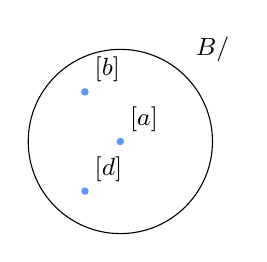
\begin{tikzpicture}[scale=.9,x=10mm,y=10mm, font=\small]
\draw (0,0) circle [x radius=1.3, y radius=1.3];

\node at (1.3,1.3) {$B/\Rel$};

\begin{scope}[fill=CornflowerBlue]
\fill  (0,0)circle (1.5pt) node[above right] {$[a]$};
\fill (-.5,.7) circle (1.5pt)node[above right] {$[b]$};
\fill(-.5,-.7) circle (1.5pt)node[above right] {$[d]$};
\end{scope}
\end{tikzpicture}

\end{center}

\osservazione Ogni volta che si ha una relazione d'equivalenza~$\Rel$ in un insieme~$A$, possiamo stabilire la seguente
catena di passaggi:
 \[\text{insieme }A\rightarrow\Rel\rightarrow\text{ partizione }P(A)=\text{ insieme quoziente }A/\Rel.\]

\ovalbox{\risolvii \ref{ese:B.32}, \ref{ese:B.33}, \ref{ese:B.34}, \ref{ese:B.35}, \ref{ese:B.36}, \ref{ese:B.37}, \ref{ese:B.38}, \ref{ese:B.39}, \ref{ese:B.40},
\ref{ese:B.41}, \ref{ese:B.42}}

\ovalbox{\ref{ese:B.43}}

\section{Relazioni di ordine}

Nel linguaggio di ogni giorno avrai certamente spesso usato espressioni come ``devo mettere in ordine i miei
libri'' oppure ``qui non c'è ordine'' e altre espressioni simili.
Anche in matematica, fin dalla scuola elementare, hai imparato a ordinare gli elementi dell'insieme dei
numeri naturali: dati due numeri naturali hai imparato infatti a stabilire quale dei due è il maggiore.

\begin{definizione}
Una relazione~$\Rel$, introdotta in un insieme~$A$, si chiama \emph{relazione d'ordine} se è antisimmetrica e transitiva.
\end{definizione}

Riguardando le varie relazioni introdotte sin qui, possiamo stabilire che esistono relazioni d'ordine di vario tipo, schematizzate nel seguente diagramma:
\begin{center}
 % (c) 2012 Dimitrios Vrettos - d.vrettos@gmail.com

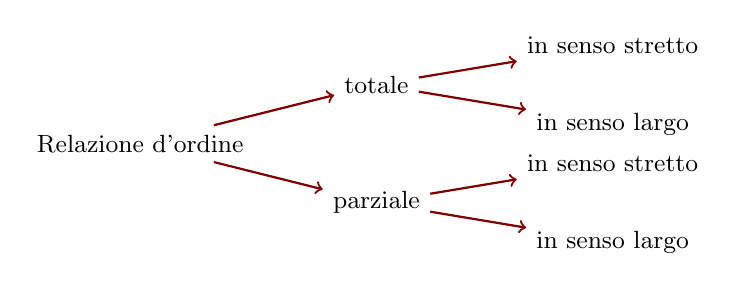
\begin{tikzpicture}[x=10mm,y=10mm, font=\small]

\node {Relazione d'ordine}[grow=right,level distance= 30mm, sibling distance=15mm,->,thick, draw=Maroon]
child {node {parziale}[sibling distance=10mm]
child {node {in senso largo}}
child {node {in senso stretto}}}
child {node {totale}[sibling distance=10mm]
child {node {in senso largo}}
child {node {in senso stretto}}};

\end{tikzpicture}

\end{center}

Attraverso alcuni esempi, vogliamo chiarire le differenze tra i diversi tipi. A questo scopo introduciamo la seguente definizione.

\begin{definizione}
Data una relazione d'ordine~$\Rel$ definita in un insieme~$A$, due elementi distinti~$x$ e~$y$ sono \emph{confrontabili} se rispetto a~$\Rel$ si ha~$x \,\Rel\, y$ oppure~$y \,\Rel\, x$.
\end{definizione}

\begin{exrig}
 \begin{esempio}

In base al diagramma di Eulero-Venn riportato nella figura~\ref{fig:B.5} a pagina~\pageref{fig:B.5}, introduciamo nell'insieme~$S = \{U$, $A$, $B$, $C$, $D$, $E$, $F\}$ la relazione~$\Rel$: ``essere sottoinsieme di''.
Ricordiamo che, dati due insiemi~$X$ e~$Y$, $X$ è \emph{sottoinsieme} di~$Y$, in simboli $X \subseteq Y$, quando ogni elemento di~$X$ appartiene a~$Y$.

Vogliamo studiare le proprietà della relazione~$\Rel$:

\begin{enumeratea}
\item poiché ogni insieme è sottoinsieme di se stesso, possiamo dire che~$\Rel$ è riflessiva;
\item se~$X \subseteq Y$ e~$X \neq Y$ allora~$Y \not\subseteq X$ quindi~$\Rel$ è una relazione antisimmetrica;
\item se~$X \subseteq Y$ e~$Y \subseteq Z$ allora~$X \subseteq Z$ quindi~$\Rel$ è una relazione transitiva.
\end{enumeratea}

Inoltre è evidente che esistono almeno due elementi dell'insieme~$S$ che non sono in
alcun modo in relazione: ad esempio~$A \not\subseteq D$ e~$D \not\subseteq A$, ossia~$A$ e~$D$ non sono confrontabili.

 \end{esempio}

 \begin{esempio}

Riprendiamo il diagramma di Eulero-Venn dell'esempio precedente e introduciamo nell'insieme~$S = \{U$, $A$, $B$, $C$, $D$, $E$, $F\}$ la relazione~$\Rel$:
``essere sottoinsieme proprio di''. Studiamo le proprietà di questa relazione:
\begin{itemize*}
 \item cosa è cambiato rispetto alla relazione precedente? $\ldots$
 \item sono ancora valide le proprietà antisimmetrica e transitiva? $\ldots$
 \item esistono elementi di~$S$ non confrontabili? $\ldots$
\end{itemize*}

 \end{esempio}
\end{exrig}

\begin{definizione}
Una relazione d'ordine si dice \emph{parziale} quando esistono almeno due elementi che non sono confrontabili.
\end{definizione}

\begin{definizione}
Una relazione d'ordine si dice \emph{totale} quando due qualsiasi elementi possono essere messi in relazione, cioè sono confrontabili.
\end{definizione}

\begin{definizione}
Una relazione d'ordine è detta \emph{in senso largo} quando essa gode della proprietà riflessiva.
\end{definizione}

\begin{definizione}
Una relazione d'ordine è detta \emph{in senso stretto} quando essa gode della proprietà antiriflessiva.
\end{definizione}

\begin{center}
 % (c) 2012 Dimitrios Vrettos - d.vrettos@gmail.com

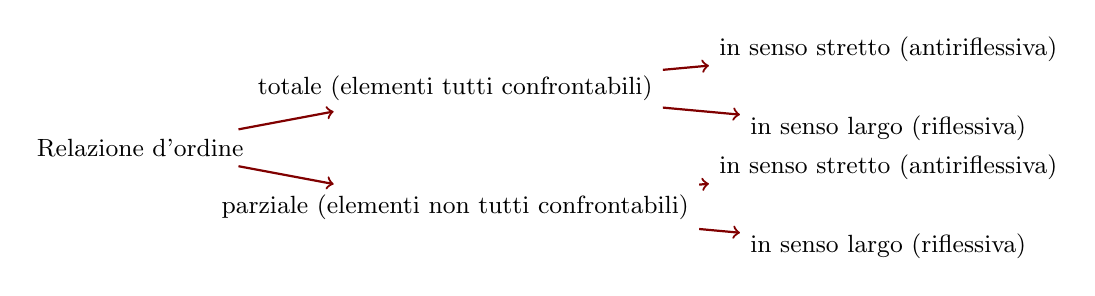
\begin{tikzpicture}[x=10mm,y=10mm, font=\small]

\node {Relazione d'ordine}[grow=right,level distance= 40mm,->,thick, draw=Maroon]
child {node {parziale (elementi non tutti confrontabili)}[level distance=55mm,sibling distance=10mm]
child {node {in senso largo (riflessiva)}}
child {node {in senso stretto (antiriflessiva)}}}
child {node {totale (elementi tutti confrontabili)}[level distance=55mm,sibling distance=10mm]
child {node {in senso largo (riflessiva)}}
child {node {in senso stretto (antiriflessiva)}}};

\end{tikzpicture}

\end{center}

\ovalbox{\risolvii \ref{ese:B.44}, \ref{ese:B.45}, \ref{ese:B.46}, \ref{ese:B.47}, \ref{ese:B.48}, \ref{ese:B.49}, \ref{ese:B.50}, \ref{ese:B.51},
\ref{ese:B.52}, \ref{ese:B.53}, \ref{ese:B.54}}

\ovalbox{ \ref{ese:B.55}, \ref{ese:B.56}, \ref{ese:B.57}, \ref{ese:B.58}, \ref{ese:B.59}, \ref{ese:B.60},
\ref{ese:B.61},\ref{ese:B.62}, \ref{ese:B.63}}
\newpage
% (c) 2012 Tiziana Manca - tmanca@libero.it
% (c) 2012-2014 Dimitrios Vrettos - d.vrettos@gmail.com
%===================================
\section{Esercizi}
%===================================
\subsection{Esercizi dei singoli paragrafi}
%===================================
\subsubsection*{\thechapter.1 - Proposizioni e predicati}

\begin{esercizio}
\label{ese:B.1}
Completa la tabella come suggerito nella prima riga, individuando, per ciascuna proposizione, il predicato e gli argomenti a cui esso si riferisce:
\begin{center}
\begin{tabular}{llc}
\toprule
Proposizioni & Predicato & Argomenti\\
\midrule
7 è divisore di~14 & essere divisore di & 7, 14 \\
11 è maggiore di~10 & essere maggiore di & \\
5 è numero primo & & \\
Andrea frequenta la stessa palestra di Marco & & \\
Marta è moglie di Piero & & \\
Paolo è padre di Marco & & \\
\bottomrule
\end{tabular}
\end{center}
\end{esercizio}


\begin{multicols}{2}
%===================================
\subsubsection*{\thechapter.2 - Relazioni in un insieme}
\begin{esercizio}
\label{ese:B.2}
Nell'insieme~$A = \{$3, 5, 6, 9, 30$\}$ considera il predicato ``essere minore di''; con esso forma proposizioni vere aventi come soggetto e come complemento due elementi di~$A$.
\begin{enumeratea}
\item $p_1$: 9\text{ è minore di }30;
\item $p_2$: \dotfill;
\item $p_3$: \dotfill
\end{enumeratea}
\end{esercizio}

\begin{esercizio}
\label{ese:B.3}
Nell'insieme~$A$ rappresentato con il diagramma di Eulero-Venn di figura~\ref{fig:B.11} a pagina~\pageref{fig:B.11} introduciamo il predicato~$\Rel$: ``avere
una sola lettera diversa''. Costruisci l'insieme~$G_\Rel$.

\emph{Traccia di soluzione}:
Per costruire l'insieme~$G_\Rel$ devo formare le coppie ordinate ricordando che per qualunque~$a$ e~$b$ appartenenti ad~$A$, $a \,\Rel\, b$
se e solo se ``$a$ ha una sola lettera diversa da~$b$'', ad esempio prete$\,\Rel\,$prese.
\end{esercizio}

\begin{esercizio}
\label{ese:B.4}
Nell'insieme~$C = \{$Como, Milano, Venezia, Parma, Brescia, Aosta, Torino, Genova, Imperia, Arezzo,
Firenze, Grosseto, Napoli, Campobasso, Catanzaro, Bologna, Vercelli, Salerno$\}$ è definita la
relazione~$\Rel$: ``essere nella stessa regione''. Costruisci l'insieme~$G_\Rel$.
\end{esercizio}

\begin{esercizio}
\label{ese:B.5}
Nell'insieme~$S = \{ x \mid  x$ è il nome di un giorno della settimana$\}$ è definita la
relazione~$\Rel$:~$x \in S$, $y \in S$, $x \,\Rel\, y$ se e solo se ``$x$ ha
lo stesso numero di sillabe di~$y$''. Costruisci l'insieme~$G_\Rel$.
\end{esercizio}

\begin{esercizio}
\label{ese:B.6}
Nell'insieme~$F = \{$1, 3, 4, 6, 5, 9, 0, 2$\}$ è definita la relazione~$\Rel$: ``essere consecutivi''. Costruisci l'insieme~$G_\Rel$.
\end{esercizio}
\end{multicols}

\begin{figure}[t]
\begin{minipage}[b]{.45\textwidth}
 \centering
 % (c) 2012 Dimitrios Vrettos - d.vrettos@gmail.com

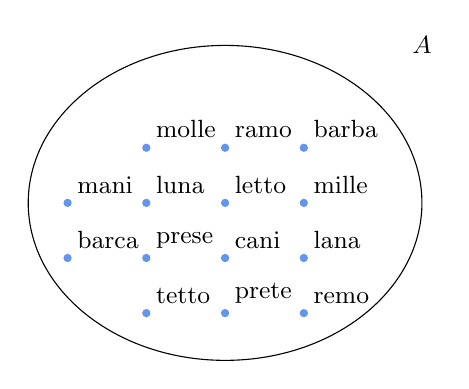
\begin{tikzpicture}[x=10mm,y=10mm, font=\small]
\draw (0,0) circle [x radius=2.5, y radius=2];

\node  at (2.5,2) {$A$};
 \begin{scope}[fill=CornflowerBlue]
\fill (0,0) circle (1.5pt) node[above right] {letto};
\fill (-1,0) circle (1.5pt) node[above right] {luna};
\fill (-2,0) circle (1.5pt) node[above right] {mani};
\fill (-2,-.7) circle (1.5pt) node[above right] {barca};
\fill (1,0) circle (1.5pt) node[above right] {mille};
\fill (0,.7) circle (1.5pt) node[above right] {ramo};
\fill (1,.7) circle (1.5pt) node[above right] {barba};
\fill (-1,.7) circle (1.5pt) node[above right] {molle};
\fill (0,-.7) circle (1.5pt) node[above right] {cani};
\fill (1,-.7) circle (1.5pt) node[above right] {lana};
\fill (-1,-.7) circle (1.5pt) node[above right] {prese}; 
\fill (0,-1.4) circle (1.5pt) node[above right] {prete};
\fill (1,-1.4) circle (1.5pt) node[above right] {remo};
\fill (-1,-1.4) circle (1.5pt) node[above right] {tetto}; 
 \end{scope}
\end{tikzpicture}
 \caption{Esercizio \ref{ese:B.3}.}\label{fig:B.11}
\end{minipage}\hfil
\begin{minipage}[b]{.45\textwidth}
 \centering
 % (c) 2012 Dimitrios Vrettos - d.vrettos@gmail.com
\begin{tikzpicture}[scale=.5, x=7.5mm, y=7.5mm, font=\scriptsize]
\begin{scope}[->]
\draw (0,0) -- (0,7.5);
\draw (0,0) -- (7.5,0);
\end{scope}

\begin{scope}[Maroon, dotted, step=7.5mm]
\draw (0,0) grid (7.5,7.5);
\end{scope}

\foreach \x/\xtext in {1/lunedì,2/martedì}{
\node[below left=.2, rotate=30] at (\x,0) {\xtext};
\node[left=.15] at (0,\x) {\xtext};
}
\begin{scope}[very thick, draw=CornflowerBlue, decoration={crosses, shape size=1.5mm}]
\draw decorate {(1,1) -- (1,1.1)};
\draw decorate {(2,2) -- (2,2.1)};
\end{scope}
\end{tikzpicture}
 \caption{Esercizio \ref{ese:B.7}.}\label{fig:B.12}
\end{minipage}
\end{figure}
\begin{multicols}{2}
%===================================
\subsubsection*{\thechapter.3 - Grafico di una relazione}
 \begin{esercizio}
\label{ese:B.7}
Considera l'insieme~$S = \{ x \mid  x$ è il nome di un giorno della settimana$\}$, completa la rappresentazione grafica di figura~\ref{fig:B.12} a pagina~\pageref{fig:B.12}, dell'insieme~$S \times S$,
evidenzia poi con una crocetta gli elementi dell'insieme~$G_\Rel$ determinato dalla relazione ``$x$ ha lo stesso numero di sillabe di~$y$''.
\end{esercizio}

\begin{esercizio}
\label{ese:B.8}
Considera l'insieme~$F = \{$1, 3, 4, 6, 5, 9, 0, 2$\}$; fai la rappresentazione grafica dell'insieme~$F \times F$ e metti in evidenza con una crocetta gli
elementi dell'insieme~$G_\Rel$ determinato dalla relazione ``essere consecutivi''.
\end{esercizio}
\end{multicols}
%\newpage

\begin{multicols}{2}
 \subsubsection*{\thechapter.4 - Matrice o tabella di una relazione}

\begin{esercizio}
\label{ese:B.9}
Considera nell'insieme~$A = \{-1$, $+3$, $-7$, $+5$, $-2$, $+4$, $+10\}$ la relazione~$\Rel$:~$x \in A$, $y \in A$, $x \Rel y$ se e solo se ``$x$
è concorde con~$y$''. Costruiamo una tabella a doppia entrata (figura~\ref{fig:B.13}) riportando in orizzontale e in verticale gli elementi dell'insieme~$A$.
Fissa l'attenzione su una cella e segui le istruzioni:
\begin{itemize*}
\item se~$a \,\Rel\, b$ metti~1 nella cella~$(a;b)$;
\item altrimenti metti~0 nella cella~$(a;b)$.
\end{itemize*}
Prosegui tu seguendo l'esempio.
\end{esercizio}

\osservazione Alla fine tutte le celle sono riempite: compare zero se gli elementi della coppia ordinata non sono in relazione, compare~1 al contrario.
La relazione~$\Rel$ è completamente rappresentata.

La tabella costruita si chiama \emph{matrice della relazione}.
Una relazione può sempre essere rappresentata attraverso una matrice.

\begin{esercizio}
\label{ese:B.10}
Nell'insieme~$S = \{ x \mid  x$ è il nome di un giorno della settimana$\}$ è introdotta la relazione~$\Rel$:~$x \in S$, $y \in S$, $x \,\Rel\, y$
se e solo se ``$x$ ha lo stesso numero di sillabe di~$y$''. Rappresenta la relazione con una matrice.
\end{esercizio}

\begin{esercizio}
\label{ese:B.11}
Assegnato il predicato~$\Rel$: ``essere divisibile per'' introdotto nell'insieme~$A =\{$12, 4, 2, 8, 3, 21, 5, 60$\}$, rappresenta con una matrice la relazione~$\Rel$.
\end{esercizio}

\end{multicols}

\begin{figure}[b]
\begin{minipage}[b]{.45\textwidth}
 \centering
 % (c) 2012 Dimitrios Vrettos - d.vrettos@gmail.com

\begin{tikzpicture}[x=10mm,y=10mm, font=\small,table nodes/.style={%
		rectangle,
		draw=black,
 		align=center,
   		minimum height=5mm,
     	text depth=0.5ex,
     	text height=1.5ex,
     	inner xsep=-1pt,
     	outer sep=0pt
	},
	table/.style={%
        matrix of nodes,
        row sep=-\pgflinewidth,
        column sep=-\pgflinewidth,
        nodes={%
            table nodes
        } }]

\matrix (first) [table,text width=7mm,name=table,row 2 column 2/.style=blue,row 5 column 4/.style=blue]
{
{}  & $-1$ & $+3$ & $-7$ & $+5$ & $-2$ & $+4$ & $+10$\\
$-1$ &[blue] 1 &{} &{} &{} &{} &{} &{} \\
$+3$ &{} &{} &{} &{} &{} &{} &{} \\
$-7$ &{} &{} &{} &{} &{} &{} &{} \\
$+5$ &{} &{} &{$0$} &{} &{} &{} &{} \\
$-2$ &{} &{} &{} &{} &{} &{} &{} \\
$+4$ &{} &{} &{} &{} &{} &{} &{} \\
$+10$ &{} &{} &{} &{} &{} &{} &{} \\
};

\end{tikzpicture}
 \caption{Esercizio \ref{ese:B.9}.}\label{fig:B.13}
\end{minipage}\hfil
\begin{minipage}[b]{.45\textwidth}
 \centering
 % (c) 2012 Dimitrios Vrettos - d.vrettos@gmail.com

\begin{tikzpicture}[x=10mm,y=10mm, font=\small, every state/.style={draw=CornflowerBlue}, every loop/.style={draw=Maroon}]
\draw (0,0) circle (2);
\node at (2,2) {$A$};
\node[state]  at (-1.5,0) {};
\node[state] (3) at (-.4,.8) {$+3$};
\node[state]  at (1.1,.5) {};
\node[state]  at (-.5,-.2) {};
\node[state] (10) at (1,-1) {$+10$};
\node[state] (7) at (-.5,-1.2) {$-7$};

\begin{scope}[->]
\path (3) edge[loop above] node{} ()
	(10) edge[loop above] node{} ()
   (7) edge[loop right] node {} ();

\end{scope}
\begin{scope}[-, Maroon]
\draw (10)--(3);
\end{scope}
\end{tikzpicture}
 \caption{Esercizio \ref{ese:B.12}.}\label{fig:B.14}
\end{minipage}
\end{figure}
%\newpage
\begin{multicols}{2}

\subsubsection*{\thechapter.5 - Grafo di una relazione}

\begin{esercizio}
\label{ese:B.12}
Completa la rappresentazione di figura~\ref{fig:B.14} a pagina~\pageref{fig:B.14} con le frecce relative alla relazione~$\Rel$:~$x \in A$, $y \in A$, $x \Rel y$ se e solo se ``$x$ è concorde con~$y$''
nell'insieme~$A =\{-1$, $+3$, $-7$, $+5$, $-2$, $+4$, $+10\}$.
\osservazione Nel completare il disegno dell'esercizio precedente hai dovuto utilizzare una freccia con due punte, infatti le proposizioni
``$+3$ è concorde con~$+10$'' e ``$+10$ è concorde con~$+3$'' sono entrambe vere. Quando si ha questo caso si possono omettere le punte
delle frecce utilizzando un semplice arco che collega gli argomenti del predicato.
\end{esercizio}

\begin{esercizio}
\label{ese:B.13}
Nell'insieme~$A = \{$1, 2, 3, 4, 5, 6, 7, 8, 9$\}$ è introdotto il predicato~$\Rel$: ``essere il
doppio di''; costruisci l'insieme~$G_\Rel$, rappresenta la relazione nei tre modi descritti sopra: con un grafico cartesiano,
con una matrice e con un grafo.
\end{esercizio}

\begin{esercizio}
\label{ese:B.14}
Sono assegnati i grafi di tre relazioni~$\Rel_1$, $\Rel_2$, $\Rel_3$ definite in altrettanti insiemi~$A$, $B$, $C$ (figura~\ref{fig:B.15}); deduci da essi gli elementi di ciascun
insieme e costruisci, per ciascuna relazione, l'insieme~$G_\Rel$.
\end{esercizio}

\begin{esercizio}
\label{ese:B.15}
Rappresenta nei tre modi che sono stati descritti (con un grafico cartesiano, con una matrice, con un
grafo) la relazione~$\Rel$: ``essere nati nello stesso mese'' introdotta nell'insieme~$C$ degli alunni della tua classe.
\end{esercizio}

\begin{esercizio}
\label{ese:B.16}
Nell'insieme~$H = \{ x \in \insN \mid  21 < x < 40 \}$, $x \,\Rel\, y$ se e solo se ``la somma delle cifre di~$x$ è uguale alla somma delle cifre di~$y$''.
Costruisci~$G_\Rel$ e rappresenta la relazione con una matrice.
\end{esercizio}

\begin{esercizio}
\label{ese:B.17}
Scegli la risposta corretta:
Una relazione $\Rel$ introdotta in un insieme~$A$ determina:
\begin{enumeratea}
 \item un sottoinsieme di~$A$;
 \item l'insieme~$A \times A$;
 \item un insieme di coppie;
 \item un grafico cartesiano;
 \item un sottoinsieme di~$A \times A$.
 \end{enumeratea}
\end{esercizio}

\begin{esercizio}
\label{ese:B.18}
Rappresenta con un grafo la relazione~$\Rel$ indicata dal grafico cartesiano riportato nella figura~\ref{fig:B.16}.
\end{esercizio}
\end{multicols}

\begin{figure}[t]
\begin{minipage}[b]{.69\textwidth}
 \centering
 % (c) 2012 Dimitrios Vrettos - d.vrettos@gmail.com

\begin{tikzpicture}[x=10mm,y=10mm, font=\small, every state/.style={draw=CornflowerBlue, minimum size=0pt}, every loop/.style={draw=Maroon}]
\draw (0,0) circle (1.5);
\node at (1.3,1.5) {$A$};
\node[state] (A) at (-1,0) {$a$};
\node[state] (B) at (.5,.5) {$b$};
\node[state] (C) at (0,-1) {$c$};

\begin{scope}[->]
\path (A) edge[loop above] node{} ()
	(B) edge[loop above] node{} ()
   (C) edge[loop right] node {} ();

\end{scope}
\begin{scope}[->, Maroon]
\draw (A)--(B);
\draw (B)--(C);
\end{scope}

\begin{scope}[xshift=31mm]
\draw (0,0) circle (1.5);
\node at (1.3,1.5) {$B$};
\node[state] (1) at (.8,.6) {$1$};
\node[state] (2) at (1.1,0) {$2$};
\node[state] (3) at (-.5,-.8) {$3$};
\node[state] (4) at (.8,-.8) {$4$};
\node[state] (5) at (-1,0) {$5$};
\node[state] (6) at (-.2,.7) {$6$};

\begin{scope}[->]
\path (6) edge[loop above] node{} ()
	(3) edge[loop left] node {} ();

\end{scope}
\begin{scope}[->, Maroon]
\draw (6)--(1);
\draw (6)--(5);
\draw (4)--(2);
\draw (4)--(3);
\draw (2)--(3);
\end{scope}
\end{scope}

\begin{scope}[xshift=62mm]
\draw (0,0) circle (1.5);
\node at (1.3,1.5) {$C$};
\node[state] (D) at (.9,.6) {$D$};
\node[state] (E) at (.7,-.8) {$E$};
\node[state] (G) at (-.5,-.7) {$G$};
\node[state] (H) at (-.7,0) {$H$};
\node[state] (I) at (-.2,.8) {$I$};

\begin{scope}[->]
\path (I) edge[loop above] node{} ()
	(H) edge[loop left] node {} ()
(G) edge[loop left] node {} ()
(E) edge[loop above] node {} ()
(D) edge[loop below] node {} ();

\end{scope}
\begin{scope}[-, Maroon]
\draw (D)--(I);
\draw (I)--(H);
\draw (D)--(H);
\draw (G)--(E);
\end{scope}
\end{scope}
\end{tikzpicture}
 \caption{Esercizio \ref{ese:B.14}.}\label{fig:B.15}
\end{minipage}\
\begin{minipage}[b]{.3\textwidth}
 \centering
 % (c) 2012 Dimitrios Vrettos - d.vrettos@gmail.com

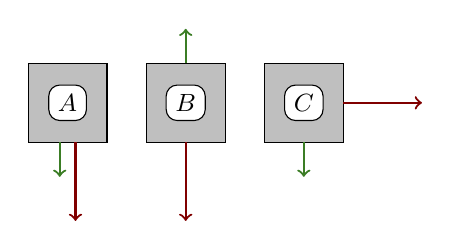
\begin{tikzpicture}[x=10mm,y=10mm, font=\small]

  \begin{scope}[fill=lightgray, draw=black]
    \foreach \x in {0, 1.5, 3}
      \filldraw (\x,0) rectangle  (\x+1,1);
  \end{scope}

  \begin{scope}[every node/.style={fill=white,rectangle, rounded corners, draw=black}]
    \foreach \x/\xtext in {.5/A,2/B,3.5/C}
      \node at (\x,.5) {$\xtext$};
  \end{scope}

  \begin{scope}[thick, ->]
    \begin{scope}[Maroon]
      \draw (.6,0) -- (.6,-1);
      \draw (2,0) -- (2,-1);
      \draw (4,.5) -- (5,.5);
    \end{scope}

    \begin{scope}[OliveGreen]
      \draw (.4,0) -- (.4,-.44);
      \draw (2,1) -- (2,1.44);
      \draw (3.5,0) -- (3.5,-.44);
    \end{scope}
  \end{scope}
\end{tikzpicture}
 \caption{Esercizio \ref{ese:B.18}.}\label{fig:B.16}
\end{minipage}
\end{figure}
\pagebreak

\subsubsection*{\thechapter.6 - Proprietà riflessiva}

\begin{esercizio}
\label{ese:B.19}
Quali relazioni sono riflessive?
\begin{center}
\begin{tabular}{llc}
\toprule
Insieme & Relazione & È riflessiva?\\
\midrule
Numeri naturali & essere divisibile per & \boxSi\quad\boxNo \\
Libri che hai in cartella & avere lo stesso numero di pagine di & \boxSi\quad\boxNo \\
Rette del piano & essere perpendicolare a & \boxSi\quad\boxNo \\
Rette del piano & essere parallela a & \boxSi\quad\boxNo \\
Poligoni & avere lo stesso numero di lati di & \boxSi\quad\boxNo \\
Città della Lombardia & terminare con la stessa vocale & \boxSi\quad\boxNo \\
Parole italiane & essere il plurale di & \boxSi\quad\boxNo \\
\bottomrule
\end{tabular}
\end{center}
\end{esercizio}

\subsubsection*{\thechapter.7 - Proprietà antiriflessiva}

\begin{esercizio}
\label{ese:B.20}
Quali delle seguenti relazioni sono antiriflessive?
\begin{center}
\begin{tabular}{llc}
\toprule
Insieme & Relazione & È antiriflessiva?\\
\midrule
Numeri naturali & essere multiplo di & \boxSi\quad\boxNo \\
Rette del piano & essere perpendicolare a & \boxSi\quad\boxNo \\
Poligoni & avere lo stesso perimetro & \boxSi\quad\boxNo \\
Città del Piemonte & avere più abitanti di & \boxSi\quad\boxNo \\
Parole italiane & essere il femminile di & \boxSi\quad\boxNo \\
Fiumi italiani & essere affluente di & \boxSi\quad\boxNo \\
Persone & essere figlio di & \boxSi\quad\boxNo \\
\bottomrule
\end{tabular}
\end{center}
\end{esercizio}

\subsubsection*{\thechapter.8 - Proprietà simmetrica}

\begin{esercizio}
\label{ese:B.21}
Riconosci le relazioni simmetriche:
\begin{center}
\begin{tabular}{llc}
\toprule
Insieme & Relazione & È simmetrica?\\
\midrule
Città d'Italia & appartenere alla stessa regione & \boxSi\quad\boxNo \\
Rette del piano & essere perpendicolare a & \boxSi\quad\boxNo \\
Solidi & avere lo stesso volume di & \boxSi\quad\boxNo \\
Persone & essere il padre di & \boxSi\quad\boxNo \\
Persone & essere fratello o sorella di & \boxSi\quad\boxNo \\
Numeri naturali & avere lo stesso numero di cifre di & \boxSi\quad\boxNo \\
Fiumi d'Europa & essere affluente di & \boxSi\quad\boxNo \\
Numeri interi & essere il quadrato di & \boxSi\quad\boxNo \\
\bottomrule
\end{tabular}
\end{center}

Le relazioni degli ultimi due casi non godono della proprietà simmetrica. Infatti:
\begin{itemize*}
\item la proposizione ``Il Ticino è un affluente del Po'' è vera, ma non lo è la proposizione che da essa si
ottiene scambiando il soggetto con il complemento;
\item se un numero intero è il quadrato di un altro (ad esempio~$+25$ è il quadrato di~$+5$), non è vero il contrario (infatti~$+5$ non è il quadrato di~$+25$).
\end{itemize*}
\end{esercizio}

\subsubsection*{\thechapter.9 - Proprietà antisimmetrica}

\begin{esercizio}
\label{ese:B.22}
Riconosci le relazioni antisimmetriche:
\begin{center}
\begin{tabular}{llc}
\toprule
Insieme & Relazione & È antisimmetrica?\\
\midrule
Numeri naturali & essere divisibile per & \boxSi\quad\boxNo \\
Rette del piano & essere perpendicolare a & \boxSi\quad\boxNo \\
Poligoni & avere lo stesso perimetro di & \boxSi\quad\boxNo \\
Angoli & essere complementare a & \boxSi\quad\boxNo \\
Città del Lazio & essere nella stessa provincia di & \boxSi\quad\boxNo \\
\bottomrule
\end{tabular}
\end{center}
\end{esercizio}

\subsubsection*{\thechapter.10 - Proprietà transitiva}

\begin{esercizio}
\label{ese:B.23}
Verifica se, nell'insieme ~$\insN$ dei numeri naturali, la relazione~$\Rel$: ``avere lo stesso numero di cifre'' gode della proprietà transitiva.
Completa le proposizioni e rappresenta~$\Rel$ con un grafo:

\begin{enumeratea}
\item da~$18 \,\Rel\,50$ e~$50 \,\Rel\, \ldots$ segue~$\ldots \,\Rel\, \ldots$;
\item da~$\ldots \,\Rel\,555$ e~$\ldots \,\Rel\,267$ segue~$\ldots \,\Rel\, \ldots$
\end{enumeratea}
\end{esercizio}

\begin{esercizio}
\label{ese:B.24}
Indica quale tra le seguenti relazioni è transitiva:
\begin{center}
\begin{tabular}{llc}
\toprule
Insieme & Relazione & È transitiva?\\
\midrule
Numeri naturali & essere multiplo di & \boxSi\quad\boxNo \\
Regioni d'Italia & essere più a nord di & \boxSi\quad\boxNo \\
Numeri interi & essere minore di & \boxSi\quad\boxNo \\
Rette del piano & essere perpendicolare a & \boxSi\quad\boxNo \\
Persone & essere padre di & \boxSi\quad\boxNo \\
Stati d'Europa & confinare con & \boxSi\quad\boxNo \\
\bottomrule
\end{tabular}
\end{center}
\end{esercizio}

\begin{esercizio}
\label{ese:B.25}
Dai una rappresentazione tabulare dell'insieme~$H = \{ x \in \insN \mid  0 \le x \le~12 \}$; determina il resto della divisione di ciascun numero di~$H$ con~4,
compila la tabella come suggerito nell'esempio:
\begin{center}
\begin{tabular}{lccccccccccccc}
\toprule
operazione & $0:4$ & $1:4$ & $2:4$ & & & & & & & & & & $12:4$ \\
resto & 0 & 1 & & & & & & & & & & & 0 \\
\bottomrule
\end{tabular}
\end{center}
Introduciamo in~$H$ la relazione~$x \,\Rel\, y$ se e solo se ``$x$ e~$y$ hanno lo stesso resto nella divisione per~4''.
Costruisci il grafo della relazione e stabilisci se gode della proprietà transitiva.

La stessa relazione~$\Rel$, introdotta nell'insieme dei numeri naturali~$\insN$ è una relazione transitiva?
\end{esercizio}

\begin{multicols}{2}
\begin{esercizio}
\label{ese:B.26}
Completa il grafo in figura~\ref{fig:B.17} a pagina~\pageref{fig:B.17} in modo che la relazione rappresentata diventi transitiva.
\end{esercizio}

\begin{esercizio}
\label{ese:B.27}
Indica la risposta corretta:

\begin{enumeratea}
\TabPositions{12cm}
\item se una relazione è simmetrica, all'insieme~$G_\Rel$ appartengono le coppie del tipo~$(a;b)$ e~$(b;a)$;
\item il grafico cartesiano è un modo per rappresentare una relazione;
\item la matrice di una relazione riflessiva presenta tutti uno sulla diagonale discendente;
\item la matrice di una relazione antiriflessiva non presenta alcun uno sulla diagonale discendente;
\item se una relazione è transitiva, allora è anche simmetrica;
\item se~$(x;y) \in G_\Rel$ e~$(y;z) \in G_\Rel$ qualche volta si ha~$(x;z) \in G_\Rel$;
\item se~$(x;y) \in G_\Rel$ si ha sempre~$(y;x) \in G_\Rel$;
\item una relazione riflessiva presenta nel suo grafo il cappio su ciascun elemento;
\item una relazione binaria è individuata da un predicato che lega due argomenti dell'insieme~$A$;
\item una relazione binaria genera un sottoinsieme del prodotto cartesiano $A \times~A$.
\end{enumeratea}
\end{esercizio}

\begin{esercizio}
\label{ese:B.28}
Con riferimento al grafico cartesiano disegnato nella figura~\ref{fig:B.18}, quale dele seguenti affermazioni è vera?

\begin{enumeratea}
\item nel suo grafo almeno un elemento non presenta il cappio;
\item la relazione è antisimmetrica;
\item la relazione è transitiva;
\item l'insieme~$G_\Rel$ è costituito dalle coppie~$(1;2)$, $(1;4)$, $(3;4)$, $(4;2)$.
\end{enumeratea}
\end{esercizio}
\end{multicols}
\begin{figure}[t]
\begin{minipage}[b]{.45\textwidth}
 \centering
 % (c) 2012 Dimitrios Vrettos - d.vrettos@gmail.com

\begin{tikzpicture}[x=10mm,y=10mm, font=\small, every state/.style={draw=CornflowerBlue, minimum size=0pt}]

\node[state] (X) at (-1,0) {$X$};
\node[state] (H) at (.5,.5) {$H$};
\node[state] (K) at (1,-1) {$K$};
\node[state] (Z) at (-.5,-1) {$Z$};

\begin{scope}[->, Maroon]
\draw (X)--(H);
\draw (X)--(Z);
\draw (H)--(K);
\end{scope}

\end{tikzpicture}

 \caption{Esercizio \ref{ese:B.26}.}\label{fig:B.17}
\end{minipage}\
\begin{minipage}[b]{.45\textwidth}
 \centering
 % (c) 2012 Dimitrios Vrettos - d.vrettos@gmail.com

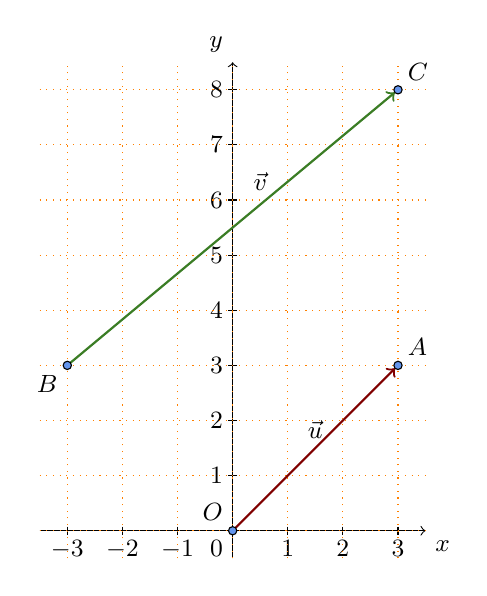
\begin{tikzpicture}[x=7mm,y=7mm, font=\small]

  \begin{scope}[->]
    \draw (-3.5,0) -- (3.5,0) node [below right] {$x$};
    \draw (0,-.5) -- (0,8.5) node[above left] {$y$};
  \end{scope}

  \foreach \x/\xtext in {-3/-3,-2/-2,-1/-1,1/1,2/2,3/3}{
    \node[below] at (\x,0) {$\xtext$};
    \draw (\x,1.5pt) -- (\x,-1.5pt);}
  \foreach \y/\ytext in {1/1,2/2,3/3,4/4,5/5,6/6,7/7,8/8}{
    \node[left] at (0,\y) {$\ytext$};
    \draw (1.5pt,\y) -- (-1.5pt,\y);}
  \node[below left] at (0,0) {$0$};

  \begin{scope}[dotted, orange, step=7mm]
    \draw (-3.5,-.5) grid (3.5,8.5);
  \end{scope}

  \begin{scope}[thick, ->,shorten >=1.5pt]
	\draw[Maroon] (0,0) -- (3,3);  
	\draw[OliveGreen](-3,3) -- (3,8);
      \end{scope}
 

\begin{scope}[fill=CornflowerBlue, draw=black]
\filldraw (0,0) circle (1.5pt)node [above left]{$O$};
\filldraw (3,3) circle (1.5pt)node [above right]{$A$};
\filldraw (-3,3) circle (1.5pt)node [below left]{$B$};
\filldraw (3,8) circle (1.5pt) node [above right]{$C$};
\end{scope}
\node[above] at (1.5,1.5) {$\vec{u}$};
\node[above] at (.5,6) {$\vec{v}$};
\end{tikzpicture}
 \caption{Esercizio \ref{ese:B.28}.}\label{fig:B.18}
\end{minipage}
\end{figure}

\begin{esercizio}
\label{ese:B.29}
Quali proprietà verificano le seguenti relazioni?
\begin{center}
(R = riflessiva, AR = antiriflessiva, S = simmetrica, AS = antisimmetrica, T = transitiva)
\end{center}
\begin{center}
\begin{tabular}{llc}
\toprule
Insieme & Relazione & Proprietà\\
\midrule
Poligoni del piano & avere lo stesso numero di lati & \boxR\quad\boxAR\quad\boxS\quad\boxAS\quad\boxT\\
Numeri naturali & avere lo stesso numero di cifre &\boxR\quad\boxAR\quad\boxS\quad\boxAS\quad\boxT\\
Numeri naturali & essere minore di &\boxR\quad\boxAR\quad\boxS\quad\boxAS\quad\boxT\\
Numeri naturali & essere divisibile per &\boxR\quad\boxAR\quad\boxS\quad\boxAS\quad\boxT\\
$A = \{ x \in \insN \mid  1 \le x \le~5 \}$ & essere multiplo di &\boxR\quad\boxAR\quad\boxS\quad\boxAS\quad\boxT\\
\bottomrule
\end{tabular}
\end{center}
\end{esercizio}

\pagebreak
\subsubsection*{\thechapter.11 - Relazioni di equivalenza}

\begin{esercizio}
\label{ese:B.30}
Quali delle seguenti sono relazioni di equivalenza?
\begin{center}
\begin{tabular}{llc}
\toprule
Relazione & Insieme & È d'equivalenza?\\
\midrule
Essere multiplo & numeri naturali & \boxV\quad\boxF \\
Avere lo stesso numero di sillabe & parole italiane & \boxV\quad\boxF\\
Essere minore & interi relativi & \boxV\quad\boxF \\
Vincere & squadre di calcio & \boxV\quad\boxF\\
Avere lo stesso numero di angoli & poligoni & \boxV\quad\boxF \\
Essere il plurale & parole italiane & \boxV\quad\boxF \\
Essere il cubo & numeri italiani & \boxV\quad\boxF \\
\bottomrule
\end{tabular}
\end{center}
\end{esercizio}
\begin{figure}[t]
 \centering% (c) 2012 Dimitrios Vrettos - d.vrettos@gmail.com

\begin{tikzpicture}[x=10mm,y=10mm, font=\small, every state/.style={draw=CornflowerBlue, minimum size=0pt}, every loop/.style={draw=Maroon}]
\draw (0,0) circle (1.5);
\node at (1.3,1.5) {$A$};
\node at (0,-2) {caso 1};
\node[state] (1) at (-1,0) {$a$};
\node[state] (2) at (.5,.7) {$b$};
\node[state] (3) at (1,0) {$c$};
\node[state] (4) at (-.6,-.7) {$d$};
\node[state] (5) at (.5,-.5) {$e$};
\node[state] (6) at (-.2,.2) {$f$};
\node[state] (7) at (.2,-1.1) {$g$};
\node[state] (8) at (-.4,1.1) {$h$};
\begin{scope}[->]
\path (1) edge[loop above] node{} ()
	(2) edge[loop above] node{} ()
   (6) edge[loop below] node {} ()
(3) edge[loop above] node{} ()
(4) edge[loop left] node{} ()
(7) edge[loop right] node{} ();

\end{scope}
\begin{scope}[-, Maroon]
\draw (1)--(8);
\draw (1)--(6);
\draw (8)--(6);

\draw (2)--(3);
\draw (2)--(5);
\draw (3)--(5);

\draw (4)--(7);
\end{scope}

 \begin{scope}[xshift=32mm]
\draw (0,0) circle (1.5);
\node at (1.3,1.5) {$B$};
\node at (0,-2) {caso 2};
\node[state] (1) at (-1,0) {$a$};
\node[state] (2) at (.5,.7) {$b$};
\node[state] (3) at (1,0) {$c$};
\node[state] (4) at (-.6,-.7) {$d$};
\node[state] (5) at (.5,-.5) {$e$};
\node[state] (6) at (-.2,.2) {$f$};
\node[state] (7) at (.2,-1.1) {$g$};
\node[state] (8) at (-.4,1.1) {$h$};
\begin{scope}[->]
\path (1) edge[loop above] node{} ()
	(2) edge[loop above] node{} ()
   (6) edge[loop below] node {} ()
(3) edge[loop above] node{} ()
(4) edge[loop left] node{} ()
(7) edge[loop right] node{} ()
(5) edge[loop right] node{} ()
(8) edge[loop right] node{} ();

\end{scope}
\begin{scope}[-, Maroon]
\draw (1)--(8);
\draw (1)--(6);
\draw (8)--(6);

\draw (2)--(3);
\draw (2)--(5);
\draw (3)--(5);

\draw (4)--(7);
\end{scope}
 \end{scope}

 \begin{scope}[xshift=64mm]
\draw (0,0) circle (1.5);
\node at (1.3,1.5) {$C$};
\node at (0,-2) {caso 3};
\node[state] (1) at (-1,0) {$a$};
\node[state] (2) at (.5,.7) {$b$};
\node[state] (3) at (1,0) {$c$};
\node[state] (4) at (-.6,-.7) {$d$};
\node[state] (5) at (.5,-.5) {$e$};

\begin{scope}[->]
\path (1) edge[loop above] node{} ()
	(2) edge[loop above] node{} ()
(3) edge[loop above] node{} ()
(4) edge[loop left] node{} ()
(5) edge[loop right] node{} ();

\end{scope}
\begin{scope}[-, Maroon]
\draw (1)--(2);
\draw (2)--(3);
\draw (4)--(5);
\end{scope}
 \end{scope}

 \begin{scope}[xshift=96mm]
\draw (0,0) circle (1.5);
\node at (1.3,1.5) {$D$};
\node at (0,-2) {caso 4};
\node[state] (1) at (-1,0) {$a$};
\node[state] (2) at (.5,.7) {$b$};
\node[state] (3) at (1,0) {$c$};
\node[state] (4) at (-.6,-.7) {$d$};
\node[state] (6) at (.5,-.5) {$f$};
\begin{scope}[->]
\path (1) edge[loop above] node{} ()
	(2) edge[loop above] node{} ()
   (6) edge[loop below] node {} ()
(3) edge[loop above] node{} ()
(4) edge[loop left] node{} ();

\end{scope}
\begin{scope}[->, Maroon]
\draw (3)--(1);
\draw (2)--(1);
\draw (2)--(3);
\end{scope}
 \end{scope}
\end{tikzpicture}
 \caption{Esercizio \ref{ese:B.31}}\label{fig:B.19}
\end{figure}

\begin{multicols}{2}
\begin{esercizio}
\label{ese:B.31}
Analizza i grafi nella figura~\ref{fig:B.19} e individua quello che rappresenta una relazione d'equivalenza:
\begin{itemize*}
\item nel caso~1 non è rappresentata una relazione d'equivalenza perché \dotfill
\item nel caso~2 la presenza del cappio su ciascun elemento indica che la relazione gode della proprietà \ldots,
il fatto che coppie di elementi siano collegate da archi indica che vale la proprietà \ldots, infine terne di elementi godono della proprietà \dotfill

In conclusione\dotfill
\item la relazione del caso~3 non gode della proprietà \dotfill, pertanto \dotfill
\item nel caso~4 sussistono le proprietà \ldots e \ldots, ma non la proprietà \ldots pertanto la relazione \dotfill
\end{itemize*}
\end{esercizio}

\begin{esercizio}
\label{ese:B.32}
Fissa l'attenzione sulla relazione~$\Rel$: ``frequentare la stessa classe'' introdotta nell'insieme~$S$ degli alunni iscritti nella tua scuola.
Verifica che~$\Rel$ è una relazione d'equivalenza. Costruisci le classi d'equivalenza. Quante ne hai potute formare? Come sono indicate nella
realtà che vivi quotidianamente? Determina la partizione~$P(S)$ in classi d'equivalenza e infine l'insieme quoziente~$S/\Rel$.
\end{esercizio}

\begin{esercizio}
\label{ese:B.33}
Studia in~$\insN$ la relazione~$\Rel$: ``avere la stessa cifra delle unità''. Verifica se è una relazione
d'equivalenza, costruisci l'insieme quoziente dopo aver risposto alle seguenti domande:\vspace{-1ex}
\begin{itemize*}
\item quanti numeri naturali sono tra loro equivalenti?
\item da quanti elementi è costituito l'insieme~$\insN/\Rel$?
\item qual è l'elemento che sceglieresti come rappresentante di ciascuna classe?
\end{itemize*}
\end{esercizio}

\begin{esercizio}
\label{ese:B.34}
Considera la relazione~$\Rel$: ``avere lo stesso resto nella divisione per due'' introdotta nell'insieme~$\insN$ e studiane le proprietà.
\begin{itemize*}
\item è una relazione d'equivalenza? Se la risposta è affermativa, costruisci l'insieme quoziente~$\insN/\Rel$.
\item quante classi d'equivalenza hai formato?
\item puoi sfruttare quanto ottenuto per enunciare le definizioni di numero pari e di numero dispari?
\item giustifica, in base allo svolgimento dell'esercizio, l'affermazione: ``L'insieme dei numeri pari è il
complementare in~$\insN$ dell'insieme dei numeri dispari''.
\end{itemize*}
\end{esercizio}

\begin{esercizio}
\label{ese:B.35}
Considera l'insieme~$A = \{x\in\insN \mid  1 \le x \le~20 \}$ e i suoi
sottoinsiemi:~$A_1 =\{$1, 5, 9, 13, 17$\}$, $A_2 =\{$2, 6, 10, 14, 18$\}$, $A_3 =\{$3, 7, 11, 15, 19$\}$, $A_4 =\{$4, 8, 12, 16, 20$\}$.
\begin{enumeratea}
\item Rappresenta gli insiemi con un diagramma di Eulero-Venn;
\item si può affermare che quei sottoinsiemi costituiscono una partizione dell'insieme~$A$?
\item è vero che a ciascuno dei suddetti sottoinsiemi appartengono i numeri di~$A$ aventi lo stesso resto nella divisione per~4?
\item quei sottoinsiemi sono dunque classi d'equivalenza? Qual è il predicato della relazione che le determina?
\end{enumeratea}
\end{esercizio}

\begin{esercizio}
\label{ese:B.36}
Nell'insieme ~$\insN$ dei numeri naturali stabilisci se è d'equivalenza la relazione~$\Rel$: ``$x \,\Rel\, y$ se e solo se~$x$ ha le stesse cifre di~$y$''.
\end{esercizio}

\begin{esercizio}
\label{ese:B.37}
Nell'insieme~$C$ degli alunni della tua classe, verifica se la relazione~$\Rel$: ``$x \,\Rel\, y$ se e solo se il cognome di~$x$ ha la stessa lettera iniziale del
cognome di~$y$'' è d'equivalenza; determina in caso affermativo la partizione dell'insieme~$C$ e l'insieme quoziente~$C/\Rel$.
\end{esercizio}

\begin{esercizio}
\label{ese:B.38}
Nell'insieme delle parole della lingua italiana verifica se la relazione ``$x \,\Rel\, y$ se e solo se~$x$ ha lo stesso numero di lettere di~$y$'' è
una relazione di equivalenza. In caso affermativo individua alcune classi di
equivalenza.
\end{esercizio}

\begin{esercizio}
\label{ese:B.39}
Nell'insieme dei nomi dei giorni della settimana considera la relazione ``$x \,\Rel\, y$ se e solo se~$x$ e~$y$ hanno almeno tre lettere in comune''.
Verifica se è una relazione di equivalenza e in caso affermativo individua le
classi di equivalenza.
\end{esercizio}

\begin{esercizio}
\label{ese:B.40}
Nell'insieme dei numeri naturali da~1 a~100, verifica se la relazione ``$x \,\Rel\, y$ se e solo se~$x$ e~$y$ hanno lo stesso numero di lettere''
è una relazione di equivalenza. Individua quante sono le classi di equivalenza.
Scrivi tutti gli elementi delle classi di equivalenza~$[1]$ e~$[10]$.
\end{esercizio}

\begin{esercizio}
\label{ese:B.41}
Nell'insieme dei numeri naturali da~1 a~100, verifica se la relazione ``$x \,\Rel\, y$ se e solo se~$x+y$ è
dispari'' è una relazione di equivalenza.
\end{esercizio}

\begin{esercizio}
\label{ese:B.42}
Nell'insieme dei nomi dei mesi dell'anno verifica se la relazione ``$x \,\Rel\, y$ se e solo se~$x$ e~$y$ hanno almeno~3 lettere in comune''
è una relazione di equivalenza. Eventualmente individua le classi di equivalenza.
\end{esercizio}

\begin{esercizio}
\label{ese:B.43}
Sia~$S$ un insieme non vuoto in cui è definita una relazione~$\Rel$ riflessiva e transitiva; in~$S$ si definisca la relazione~$\sharp$ ponendo,
per ogni~$x$, $y$ appartenenti a~$X$, $x \,\sharp\, y$ se e solo se~$x \,\Rel\, y$ e~$y \,\Rel\, x$. Verificare che~$\sharp$ è una relazione di equivalenza in~$X$.
\end{esercizio}
\end{multicols}

\begin{figure}[t]
\begin{minipage}[b]{.45\textwidth}
 \centering
 % (c) 2012 Dimitrios Vrettos - d.vrettos@gmail.com

\begin{tikzpicture}[x=10mm,y=10mm, font=\small, every state/.style={draw=CornflowerBlue, minimum size=0pt}, every loop/.style={draw=Maroon}]
\draw (0,0) circle (1.5);
\node at (1.5,1.5) {$T$};
\node[state] (1) at (-.6,.7) {$M$};
\node[state] (2) at (1,.5) {$Z$};
\node[state] (3) at (1,-.5) {$W$};
\node[state] (4) at (-.8,-.7) {$J$};
\node[state] (5) at (0.1,-1.1) {$P$};

\begin{scope}[->, Maroon]
 \draw (1)--(3);
 \draw (1)--(2);
 \draw (2)--(3); 
 \draw (2)--(5); 
 \draw (2)--(4); 
 \draw (3)--(4);
 \draw (5)--(4);
 \draw (5)--(3);
 \draw (1)--(4);
 \draw (1)--(5);
\end{scope}

\end{tikzpicture}

 \caption{Esercizio \ref{ese:B.45}.}\label{fig:B.20}
\end{minipage}\
\begin{minipage}[b]{.45\textwidth}
 \centering
 % (c) 2012 Dimitrios Vrettos - d.vrettos@gmail.com

\begin{tikzpicture}[x=10mm,y=10mm, font=\small]
 \tkzDefPoint(0,0){A}
 \tkzDefShiftPoint[A](30:4.67){C}
 \tkzDefShiftPoint[A](0:5.97){B}

 \tkzMarkAngle[fill=LimeGreen, draw=black, size=.4](B,A,C)
 \tkzMarkAngle[fill=LimeGreen, draw=black, size=.4](C,B,A)

\tkzDrawLine[add=0 and 0, thin,dashed](A,B)
\tkzDrawLine[add=0 and 0, thin](A,C)
\tkzDrawLine[add=0 and 0, thin](B,C)

 \tkzLabelPoints[below](A,B)
\tkzLabelAngle[](B,A,C){$30^\circ$}
\tkzLabelAngle[](C,B,A){$50^\circ$}
 \tkzDrawPoints[color=CornflowerBlue](A,B,C)
 
\end{tikzpicture}
 \caption{Esercizio \ref{ese:B.47}.}\label{fig:B.21}
\end{minipage}
\end{figure}

\begin{multicols}{2}
\subsubsection*{B.12 - Relazioni di ordine}
\begin{esercizio}
\label{ese:B.44}
Nell'insieme~$M =\{$1, 8, 3, 4, 10, 2, 7, 0, 5, 9, 6$\}$ viene introdotta la relazione~$\Rel$ così definita: ``$x \,\Rel\, y$ se e solo se~$y-x$ appartiene a ~$\insN$''.
La relazione è riflessiva? La relazione è antisimmetrica? La relazione è transitiva? \`E vero che due elementi
distinti sono sempre confrontabili?
\end{esercizio}

\begin{esercizio}
\label{ese:B.45}
\`E assegnata la relazione~$R$ nell'insieme~$T$, rappresentata col grafo di figura~\ref{fig:B.20}.
Analizzando il grafo, rispondi alle domande:
\begin{itemize*}
\item la relazione è riflessiva?
\item la relazione è antisimmetrica?
\item la relazione è transitiva?
\item due elementi distinti sono sempre confrontabili?
\end{itemize*}
Alla prima domanda avrai risposto negativamente: nessun elemento dell'insieme~$T$ è in relazione con se stesso, mentre valgono le proprietà antisimmetrica e transitiva.
Infine scelti due elementi qualsiasi dell'insieme~$T$, essi sono sempre confrontabili.
\end{esercizio}

\begin{esercizio}
\label{ese:B.46}
Verifica che la relazione~$\Rel$: ``essere divisore'' introdotta nell'insieme~$J =\{$3, 6, 10, 15, 21$\}$ è una relazione d'ordine parziale in senso largo.
\end{esercizio}

\begin{esercizio}
\label{ese:B.47}
Perché la relazione~$\Rel$ rappresentata dal grafico cartesiano riportato nella figura~\ref{fig:B.21}, pur essendo una relazione d'ordine non può essere
classificata in nessuna delle tipologie studiate? Dai una breve motivazione indicando quali proprietà non sono soddisfatte dalla relazione rappresentata.
\end{esercizio}

\begin{esercizio}
\label{ese:B.48}
Nell'insieme degli studenti della tua classe determina le proprietà della relazione~$\Rel$: ``$x \,\Rel\, y$ se e solo se l'altezza di~$x$ non supera l'altezza di~$y$''. \`E una relazione d'ordine? Di quale tipo?
\end{esercizio}

\begin{esercizio}
\label{ese:B.49}
Nell'insieme~$A = \{$12, 4, 2, 8, 3, 21, 5, 60$\}$ la relazione~$\Rel$: ``essere divisibile'' è una relazione d'ordine? Se lo è, di che tipo di relazione si tratta? Totale, parziale, in senso largo, in senso stretto?
\end{esercizio}

\begin{esercizio}
\label{ese:B.50}
Nell'insieme ~$\insN - \{ 0 \}$ la relazione ``essere divisibile'' è d'ordine totale in senso largo?
\end{esercizio}

\begin{esercizio}
\label{ese:B.51}
Rappresenta nelle tre modalità studiate una relazione che sia solo simmetrica; ripeti le rappresentazioni per una relazione che sia almeno simmetrica. Quale significato hanno le due richieste formulate sopra?
\end{esercizio}

\begin{esercizio}
\label{ese:B.52}
L'insieme~$G_\Rel$ di una relazione introdotta nell'insieme~$A = \{a$, $b$, $c$, $d$, $e\}$ è~$G_\Rel = \{ (a;a)$, $(a;b)$, $(b;b)$, $(d;d)$, $(c;d)$, $(d;e)$, $(e;e)\}$.
Quale delle seguenti affermazioni è vera
\begin{enumeratea}
\item $\Rel$ è una relazione antiriflessiva;
\item $\Rel$ è una relazione solo antisimmetrica;
\item $\Rel$ è una relazione riflessiva;
\item $\Rel$ è una relazione transitiva e antisimmetrica;
\end{enumeratea}
\end{esercizio}

\begin{esercizio}
\label{ese:B.53}
La relazione~$\Rel$: ``essere vicini di banco'' inserita nell'insieme degli alunni della tua classe è una
relazione d'equivalenza? \`E una relazione d'ordine?
\end{esercizio}

\end{multicols}

\begin{figure}[t]
\begin{minipage}[b]{1\textwidth}
 \centering
 % (c) 2012 Dimitrios Vrettos - d.vrettos@gmail.com

\begin{tikzpicture}[x=10mm,y=10mm, font=\small, every state/.style={draw=CornflowerBlue, minimum size=0pt}, every loop/.style={draw=Maroon}]
\draw (0,0) circle (1.5);
\node at (0,-2) {1};
\node[state] (1) at (-.6,.7) {$-12$};
\node[state] (2) at (.5,.5) {$-1$};
\node[state] (3) at (.5,-.8) {$-15$};
\node[state] (4) at (-.6,-.7) {$-7$};

\begin{scope}[->, Maroon]
 \draw (3)--(1);
 \draw (1)--(2);
 \draw (3)--(2); 
 \draw (3)--(4);
\draw (4)--(2);
 \draw (1)--(4);
\end{scope}

 \begin{scope}[xshift=31mm]
\draw (0,0) circle (1.5);
\node at (0,-2) {2};
\node[state] (1) at (-1,0) {$a$};
\node[state] (2) at (.5,.7) {$b$};
\node[state] (3) at (.5,-.5) {$c$};
\node[state] (4) at (-.6,-.7) {$m$};

\begin{scope}[->]
\path (1) edge[loop above] node{} ()
	(2) edge[loop above] node{} ()
(3) edge[loop below] node{} ()
(4) edge[loop left] node{} ();

\end{scope}
\begin{scope}[->, Maroon]
\draw (1)--(3);
\draw (1)--(2);
\draw (2)--(3);
\end{scope}
 \end{scope}

 \begin{scope}[xshift=62mm]
\draw (0,0) circle (1.5);
\node at (0,-2) {3};
\node[state] (1) at (-1,0) {$M$};
\node[state] (2) at (0,.8) {$B$};
\node[state] (3) at (1,0) {$C$};
\node[state] (4) at (0,-1) {$F$};


\begin{scope}[->]
\path (1) edge[loop above] node{} ()
	(2) edge[loop above] node{} ()
(3) edge[loop above] node{} ()
(4) edge[loop left] node{} ();

\end{scope}
\begin{scope}[->, Maroon]
\draw (1)--(2);
\draw (1)--(3);
\draw (1)--(4);
\draw (2)--(4);
\draw (4)--(3);
\end{scope}
 \end{scope}
\end{tikzpicture}
 \caption{Esercizio \ref{ese:B.58}.}\label{fig:B.22}
\end{minipage}
\hfill
\begin{minipage}[b]{\textwidth}
 \centering
 % (c) 2012 Dimitrios Vrettos - d.vrettos@gmail.com

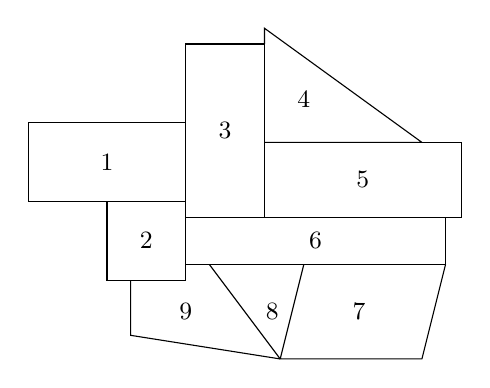
\begin{tikzpicture}[x=10mm,y=10mm, font=\small]
\draw (0,0) rectangle  (2,1) node[midway] {1};
\draw (1,-1) rectangle  (2,0) node[midway] {2};
\draw (2,-.2) rectangle  (3,2) node[midway] {3};
\draw (3,2)-- (3,2.2) -- (5,.75) --(3,.75);
\draw (3,.75) rectangle  (5.5,-.2) node[midway] {5};
\draw (2,-.2) rectangle  (5.3,-.8) node[midway] {6};
\draw (5.3,-.8) -- (5,-2) --(3.2,-2) --(3.5,-.8);
\draw (3.2,-2) -- (2.3,-.8);
\draw (3.2,-2) -- (1.3,-1.7)-- (1.3,-1);
 \node at (3.5,1.3) {4};
 \node at (4.2,-1.4) {7};
 \node at (3.1,-1.4) {8};
 \node at (2,-1.4) {9};
\end{tikzpicture}
 \caption{Esercizio \ref{ese:B.62}.}\label{fig:B.23}
\end{minipage}
\end{figure}

\begin{multicols}{2}

\begin{esercizio}
\label{ese:B.54}
I tre sottoinsiemi~$A_1 = \{$36, 135, 432$\}$, $A_2 = \{65\}$ e $A_3 = \{$66, $3\,522$, 93, 435$\}$ dell'insieme~$A = \{$36, 65, 66, 93, 135, 432, 435, $3\,522\}$ costituiscono una partizione dell'insieme~$A$? Sapresti trovare una caratteristica per gli elementi di ciascun sottoinsieme? $A_1$, $A_2$, $A_3$ sono classi d'equivalenza?
\end{esercizio}

\begin{esercizio}
\label{ese:B.55}
Nell'insieme ~$\insN$ la relazione~$\Rel$: ``$x \,\Rel\, y$ se e solo se~$x \cdot y$ è un numero dispari'' è d'equivalenza?
\end{esercizio}

\begin{esercizio}
\label{ese:B.56}
La relazione~$\Rel$: ``$x \,\Rel\, y$ se e solo se~$x$ sta nella stessa nazione di~$y$'' nell'insieme~$K= \{$Parigi, Madrid, Milano, Siviglia, Bari, Granada, Venezia, Lione$\}$
è d'equivalenza? Costruisci~$A/\Rel$.
\end{esercizio}

\begin{esercizio}
\label{ese:B.57}
Verifica se la relazione~$\Rel$ assegnata con la matrice rappresentata
sotto è d'equivalenza. In caso positivo determina la partizione dell'insieme~$A =\{\square, \lozenge, \infty, \nabla\}$ e l'insieme
quoziente~$A/\Rel$.

\begin{center}
\begin{tabular}{ccccc}
\toprule
 & $\square$ & $\lozenge$ & $\infty$ & $\nabla$\\
\midrule
 $\square$ & 1 & 1 & 0 & 0 \\
 $\lozenge$ & 1 & 1 & 0 & 0 \\
 $\infty$ & 0 & 0 & 1 & 1\\
 $\nabla$ & 0 & 0 & 1 & 1\\
\bottomrule
\end{tabular}
\end{center}
\end{esercizio}

\begin{esercizio}
\label{ese:B.58}
In un torneo di pallavolo gareggiano quattro squadre A, B, C, D; rappresenta con un grafo a frecce le seguenti informazioni, relative alle prime tre giornate:
\begin{itemize*}
\item 1\textsuperscript{a} giornata: A vince contro B; C vince contro D;
\item 2\textsuperscript{a} giornata: D vince contro A; B vince contro C;
\item 3\textsuperscript{a} giornata: A vince contro C; B vince contro D;
\end{itemize*}
Il~4\textsuperscript{o} giorno si gioca la semifinale tra le prime due classificate e le altre due. Se per ogni vittoria si ottiene un punteggio di~10 punti e per ogni sconfitta un punteggio
di~2 punti, quale squadra gioca la semifinale con B?
Il torneo è vinto dalla squadra C. Rappresenta con un grafo a frecce la situazione della semifinale e quella
della finale. \`E unica la risposta a quest'ultimo quesito?
\end{esercizio}

\begin{esercizio}
\label{ese:B.59}
Associa a ciascun grafo della figura~\ref{fig:B.22} a pagina~\pageref{fig:B.22} la corretta relazione d'ordine:
\begin{enumeratea}
\item ordine totale in senso largo;
\item ordine totale in senso stretto;
\item ordine parziale in senso largo;
\item ordine parziale in senso stretto.
\end{enumeratea}
\end{esercizio}

\begin{esercizio}
\label{ese:B.60}
Nell'insieme di tutti gli iscritti a Facebook, determina le proprietà della relazione~$\Rel$: ``$x \,\Rel\, y$ se e solo se il numero di amici di~$x$ supera
il numero di amici di~$y$''. \`E una relazione d'ordine? Se sì, di quale tipo?
\end{esercizio}

\begin{esercizio}
\label{ese:B.61}
Nell'insieme delle parole della lingua italiana, verifica se la relazione ``$x \,\Rel\, y$ se e solo se~$x$ ha più lettere di~$y$'' è una relazione d'ordine.
In caso affermativo dire se è totale o parziale, in senso largo o in senso stretto.
\end{esercizio}

\begin{esercizio}
\label{ese:B.62}
Nell'insieme dei numeri naturali, verifica se la relazione ``$x \,\Rel\, y$ se e solo se~$x$ ha un numero di cifre maggiore del numero di cifre di~$y$''
è una relazione d'ordine. In caso affermativo dire se è totale o parziale, in senso largo o in senso stretto.
\end{esercizio}

\begin{esercizio}
\label{ese:B.63}
Andrea, insegnante di grafica, ha chiesto ai suoi alunni di usare il minimo numero di colori per colorare il modello della figura~\ref{fig:B.23} a pagina~\pageref{fig:B.23},
in modo che poligoni confinanti non risultino con lo stesso colore. Come si può risolvere il problema? [Risposta: 3 colori]

\emph{Traccia di soluzione}: Nell'insieme~$Z =\{$1, 2, 3, 4, 5, 6, 7, 8, 9$\}$ studia la relazione~$\Rel$: ``confinare con'', rappresentandola con un grafico cartesiano e sfrutta
i risultati trovati per risolvere il problema.
La soluzione può essere trovata fissando un punto interno a ciascuna regione: due punti sono uniti se e solo se le regioni confinano, il segmento che li congiunge
deve attraversare solo il loro confine comune; i punti che non sono congiunti indicano regioni che avranno lo stesso colore.
\end{esercizio}
\end{multicols}

\cleardoublepage
